\seccion{Unas identidades y desigualdades}
\label{Sec:SZ:Desigualdades}

% Libro Loss Ruskai [Lieb]

\SZ{Desigualdades de Fano? Rioul p.  78, Cover P.~663, Sanov? Pythagorean? Gene:
  cf Zyc p60}

% ================================= MaxEnt

\subseccion{El principio de entrop\'ia m\'axima}
\label{Ssec:SZ:MaxEnt}

En  la  termodin\'amica, el  estudio  de  las caracter\'isticas  macrosc\'opicas
(din\'amica de las mol\'eculas) es prohibitivo tan el n\'umero de mol\'eculas es
importante. Por  ejemplo, un litro del  gas que respiramos  contiene $2.7 \times
10^{22}$  mol\'eculas.   De  esta  constataci\'on  se  desaroll\'o  la  f\'isica
estad\'isticas    bajo   el    impulso    de   Boltzmann~\cite{Bol96,    Bol98},
Maxwell~\cite{Max67},  Gibbs~\cite{Gib02}, Planck~\cite{Pla15} entre  otros (ver
tambi\'en~\cite[y   ref.]{Jay65,  Mer10,   Mer18}),   considerando  el   sistema
macrosc\'opico  a  trav\'es de  lo  que  llamaron  ensembles estad\'isticos:  el
sistema  global  (macrosc\'opico)  es  al equilibrio  pero  las  configuraciones
(micro-estados)  son  fluctuantes.   De  una  forma,  se  puede  asociar  a  una
configuraci\'on su  frecuencia de ocurrencia (imaginando tener  une infinidad de
copias del sistema en el  mismo estado macrosc\'opico), es decir su probabilidad
de  occurencia.   En  este  marco,  la  entrop\'ia,  describiendo  la  falta  de
informaci\'on, juega un  rol fundamental.  Un sistema sujeto  a v\'inculos, como
por  ejemplo teniendo  una energ\'ia  dada, debe  estar en  sus estado  lo m\'as
desorganizado dados  los v\'inculos.  En su  marco, se introdujo  la noci\'on de
entrop\'ia  termodin\'amica,  pero la  misma  es  tremendamente  vinculada a  la
entrop\'ia    de   Shannon~\footnote{Ver   ep\'igrafe    del   cap\'itulo\ldots}
(claramente, identificando las frecuencias  a probabilidades de ocurrencia).  En
otro  terminos, la  distribuci\'on describiendo  los micro-estados  debe  ser de
entrop\'ia m\'axima,  dados los  v\'inculos.  Por ejemplo,  en un  gas perfecto,
donde las part\'iculas no interactuan  (aparte chocandose), la energ\'ia es dada
por las velocidades (suma de las energ\'ias cin\'eticas individuales).  Dada una
energ\'ia  fija, la  distribuci\'on  de  las velocidad  debe  ser de  entrop\'ia
m\'axima  sujeto  a  la  energ\'ia  dada  (nada m\'as  que  la  energ\'ia  va  a
``organizar''  las  configuraciones posibles).   Intuitivamente,  en un  sistema
aislado  de  $N$ part\'iculas,  las  configuraciones  van  a ser  equiprobables,
precisamente  la   distribuci\'on  maximizando   la  entrop\'ia.   \SZ{   En  la
  subsecci\'on Sec.~\ref{Ssec:SZ:GasPerfecto}  se va a desarollar  un poco m\'as
  este ejemplo.}

De manera general, el problema se  formaliza como la b\'usqueda de la entrop\'ia
m\'axima  sujeto  a  v\'inculos.    Si  este  principio  naci\'o  en  mec\'anica
estad\'istica  (ver  tambi\'en~\cite{Jay57,   Jay57:2,  Jay65,  Mer10,  Mer18}),
encontr\'o  un  echo en  varios  campos:  en  inferencia bayesiana  para  elegir
distribuciones       del        a       priori~\footnote{Ver       nota       de
  pie~\footref{Foot:SZ:BayesPrior}.  En la  inferencia bayesiana de un parametro
  modelizado  como   aleatorio  $\theta$,  para   eligir  la  ley  a   priori  \
  $p_\Theta(\theta)$,  si se conocen  momentos por  una raz\'on  o una  otra, se
  puede elegir esta distribuci\'on como la ``menos informativa'' posible, \ie de
  entrop\'ia  m\'axima dados  los  momentos.}  conociendo  unos  momentos de  la
ley~\cite{Rob07,  Jay68,  Jay82,  Csi91},  hacer  estimaci\'on  espectral  o  de
procesos     estocasticos      autoregresivos~\cite{Bur67,     Bur75,     Jay82}
o~\cite[cap.~12]{CovTho06}, entre otros~\cite[\& ref.]{Arn01, Kap89, KapKes92}.

Sea \ $X$ \ variable aleatoria viviendo sobre (de distribuci\'on de probabilidad
de soporte) \ $X(\Omega) = \X \subseteq \Rset^d$  \ con \ $K \ge 0$ \ momentos \
$\Esp\left[ M_k(X) \right] = m_k$ \ fijos, con $M_x: \X \to \Rset$. Suponemos de
que $X$ tiene una densidad \ $p$ \ con respeto a una medida $\mu$, basicamente \
$\mu_L$ \ en el contexto continuo y $\mu_\X$ en el caso discreto. El problema de
entrop\'ia  m\'axima   se  formula  de   la  manera  siguiente:  sean   \  $M(x)
=  \begin{bmatrix} 1  &  M_1(x) &  \cdots &  M_K(x)  \end{bmatrix}^t$ \  y \  $m
= \begin{bmatrix} 1 & m_1 & \cdots & m_K \end{bmatrix}^t$ (si $K = 0, \: M = m =
1$), \ se busca,
%
\[
p^* = \argmax_p H(p) \qquad \mbox{sujeto a} \qquad p \ge 0, \quad \int_\X M(x)
\, p(x) \, d\mu(x) = m,
\]
%
donde los dos primeros v\'inculos (positividad, normalizaci\'on) aseguran de que
$p^*$ sea una distribuci\'on de probabilidad. En el ejemplo del gas perfecto, $K
= 1, \, M_1(x) = \sum_i  x_i^2$ \ (los $x_i$ son las velocidades). Introduciendo
factores  de  Lagrange  $\eta =  \begin{bmatrix}  \eta_0  &  \eta_1 &  \cdots  &
  \eta_K  \end{bmatrix}^t$ para  tener  en cuenta  los  v\'inculos, el  problema
variacional   consiste  a   resolver~\cite{GelFom63,  Bru04,   Mil00,  CamMar09,
  CovTho06}
%
\[
p^* = \argmax_p  \int_\X \left( - p(x)  \log p(x) + \eta^t M(x)  \, p(x) \right)
d\mu(x),
\]
%
donde $\eta$  ser\'a determinado para satisfacer  a los v\'inculos.   En el caso
continuo $\mu  = \mu_L$ se  usa la ecuaci\'on  de Euler-Lagrange~\cite{GelFom63,
  Bru04}, esquematicamente anulando la ``derivada'' del integrande con respeto a
$p$; en  el caso  discreto, se anula  realmente un  gradiente con respeto  a los
componentes de $p$. Reparametrizando los factores de Lagrange, se obtiene as\'i
%
\[
p^*(x) = \e^{\eta^t M(x)},
\]
%
con $\eta$ tal  que se satisfacen los v\'inculos  de normalizaci\'on y momentos.
Esta  distribuci\'on   cae  en  la  familia  exponencial   que  \SZ{hemos  visto
  secci\'on~\ref{Sec:MP:}}, donde los $M_k$ son las estad\'isticas suficientes y
los $\eta_k$ los par\'ametros naturales.

Un problema que  puede aparecer es que  no se puede determinar $\eta$  tal que se
satisfacen  todos los  v\'inculos,  en particular  la  de normalizaci\'on.   Por
ejemplo,  si $\X  = \Rset$  y $K  = 0$,  \ $p$  \ deber\'ia  ser  constante (ley
uniforme) sobre\ldots $\Rset$, lo que no es normalizable. De la misma manera, si
$K  =  3$  \  y  \   $M_k(x)  =  x^k$,  tampoco  es  normalizable  la  funci\'on
obtenida~\footnote{En el  enfoque Bayesiano se puede que  no sea problem\'atico,
  si el  a posteriori es normalizable~\cite{Rob07},  pero va m\'as  all\'a de la
  meta de  esta secci\'on.}.  En  otros terminos, en  este caso, el  problema no
tiene soluci\'on~\footnote{M\'as  precisamente, existen  casos en los  cuales se
  puede acotar la entrop\'ia por arriba  por un $H^{\sup}$, tal que $\sup_p H(p)
  \le H^{\sup}$ pero no  se puede alcanzar esta cota, \ie es  un supremum, no un
  m\'aximo~\cite[sec.~12.3]{CovTho06}.}.

Existe   una  prueba   informacional   de  este   resultado,   saliendo  de   la
soluci\'on.
%
\begin{lema}
\label{Lem:SZ:MaxEntPruebaInfo}
%
  Sea  \ $\displaystyle  \P_m =  \left\{ p  \ge 0:  \: \int_\X  M(x) \,  p(x) \,
    d\mu(x) = m \right\}$ \ conjunto  de densidades con respeto a $\mu$, con los
  mismos momentos $M$, y sea \ $p^* \in  \P_m$ \ que sea de la forma \ $p^*(x) =
  \e^{\eta^t M(x)}$. Entonces
  %
  \[
  \forall \,  p \in \P_m, \quad  H(p) \le H(p^*) \qquad  \mbox{con igualdad ssi}
  \quad p = p^* \quad \mu\mbox{-(c. s.)},
  \]
  %
  donde   $H$  es   de  la   definici\'on   general  Def.~\ref{Def:SZ:ShanonMu},
  pagina~\pageref{Def:SZ:ShanonMu}, de la entrop\'ia con respeto a $\mu$.
\end{lema}
%
\begin{proof}
  \begin{eqnarray*}
  H(p) & = & - \int_\X p(x) \, \log p(x) \, d\mu(x)\\[2.5mm]
  %
  & = & - \int_\X p(x) \, \log\left( \frac{p(x)}{p^*(x)} \right) \, d\mu(x) - \int_\X
  p(x) \, \log p^*(x) \, d\mu(x)
  \end{eqnarray*}
  %
  De $\log p^* = \eta^t M$ se obtiene
  %
  \begin{eqnarray*}
  H(p) & = & - \Dkl[p]{p^*} - \int_\X \eta^t M(x) p(x)
  \, d\mu(x)\\[2.5mm]
  %
  & = & - \Dkl[p]{p^*} - \int_\X \eta^t M(x) \, p^*(x) \, d\mu(x)\\[2.5mm]
  %
  & = & - \Dkl[p]{p^*} - \int_\X p^*(x) \log p^*(x) \, d\mu(x)\\[2.5mm]
  %
  & = & - \Dkl[p]{p^*} + H(p^*)
  \end{eqnarray*}
  %
  porque $p, p^* \in \P_m$ \ (segunda  linea) y \ $\eta^t M = \log p^*$ (tercera
  linea). La prueba se cierra notando que $\Dkl[p]{p^*} \ge 0$ con igualdad si y
  solamente si $p = p^* \quad (\mu$-c.s.).
\end{proof}
%
Este lema prueba que, dados  v\'inculos ``razonables'', la entrop\'ia es acotada
por  arriba, y que  se alcanza  la cota  para una  distribuci\'on de  la familia
exponencial. Por ejemplo,
%
\begin{itemize}
\item Con  $K =  0$ \  y \  $\X$ \ de  volumen finito  \ $|\X|  < +  \infty$, la
  distribuci\'on  de entrop\'ia  m\'axima es  la distribuci\'on  uniforme  de la
  propiedad~\ref{Prop:SZ:cotamaximauniforme}      \     de      la     subsecci\'on
  Sec.~\ref{Ssec:SZ:Diferencial}      en       el      caso      continuo,      o
  propiedad~\ref{Prop:SZ:cotamaxima}        \       de        la       secci\'on
  Sec.~\ref{Ssec:SZ:DefinicionShannon} en el caso discreto.
%
\item Con $K = 1$,  \ $\X = \Rset^d$ \ y \ $M(x) = x  x^t$ (visto como $K = d^2$
  momentos),  la  distribuci\'on de  entrop\'ia  m\'axima  es la  distribuci\'on
  gausiana de  la propiedad~\ref{Prop:SZ:cotamaximagaussiana} \  de la secci\'on
  Sec.~\ref{Ssec:SZ:Diferencial}.
\end{itemize}
%
Con el enfoque del lema~\ref{Lem:SZ:MaxEntPruebaInfo}, se necesita solamente que
$p$  sea una  densidad  con respeto  a  una medida  $\mu$  fija, cualquiera.  En
particular, si es una medida de probabilidad (de referencia) $\widetilde{P}$, el
problema de entrop\'ia  m\'axima vuelve ser un problema  de minimizaci\'on de la
divergencia de Kullback-Leibler entre $P$  y la medida de referencia, siendo $p$
la    densidad    con    respeto     a    esta    medida    (ver    definici\'on
Def.~\ref{Def:SZ:entropiarelativa}). Es decir, tomando \ $\mu = \widetilde{P}$ \
medida   de   probabilidad   aparece   inmediatamente
%
\[
P^* = \argmax_P \Dkl[P]{\widetilde{P}}  \quad \mbox{sujeto a} \quad \int_\X M(x)
\,  dP(x) =  m  \qquad \Leftrightarrow  \qquad \frac{dP^*}{d\widetilde{P}}(x)  =
\e^{\eta^t x}.
\]

% ================================= EPI

\subseccion{Desigualdad de la potencia entr\'opica}
\label{Ssec:SZ:EPI}

Sean  $X$ e  $Y$  dos variables  independientes.   Si se  conoce las  relaciones
vinculando \  $H(X,Y)$, \  $H(X)$, \ $H(Y)$,  una pregunta natural  concierna la
relaci\'on  que podr\'ia  tener \  $X+Y$  \ con  cada variable  en t\'ermino  de
entrop\'ia. La respuesta no es trivial, y el resultado general concierna el caso
de  variables continuas  sobre $\Rset^d$.   Es conocido  como desigualdad  de la
potencia entr\'opica (EPI para entropy power inequality en ingl\'es). No vincula
las entrop\'ias, sino que las potencias entr\'opicas.
%
\begin{teorema}[Desigualdad de la potencia entr\'opica]
\label{Teo:SZ:EPI}
%
  Sean  $X$  e $Y$  dos  variables  $d$-dimensionales continuas  independientes.
  Entonces
  %
  \[
  N(X + Y) \ge N(X) + N(Y),
  \]
%
  con igualdad si y  solamente si \ $X$ \ e \ $Y$  \ son gaussianas con matrices
  de covarianza proporcionales, $\Sigma_Y \propto \Sigma_X$.
  % (siempre  verdad en  el contexto  escalar).
\end{teorema}
%
\noindent     Existen    varias     formulaciones     alternativas    a     esta
desiguladad~\cite{Sha48, Lie78, CovTho06, DemCov91, Rio07}:
%
\begin{enumerate}
\item\label{EPI:SZ:EquivGauss} Sean  \ $\widetilde{X}$  \ y \  $\widetilde{Y}$ \
  gaussianas independientes  de matrices de covarianza proporcionales  y tal que
  $H(\widetilde{X}) = H(X)$ y $H(\widetilde{Y}) = H(Y)$.  Entonces
  %
  \[
  N(X+Y) \ge N\left( \widetilde{X} + \widetilde{Y} \right),
  \]
  %
  con igualdad si y solamente si \ $X$  \ y \ $Y$ \ son gaussianas. De hecho, la
  primera  formulaci\'on  es equivalente  a  $N(X+Y)  \ge N\left(  \widetilde{X}
  \right) +  N\left( \widetilde{Y}  \right) = \frac{1}{2  \pi \e}  \left( \left|
      \Sigma_{\widetilde{X}}  \right|^{\frac1d} +  \left| \Sigma_{\widetilde{Y}}
    \right|^{\frac1d}     \right)    \ge     \frac{1}{2    \pi     \e}    \left|
    \Sigma_{\widetilde{X}} +  \Sigma_{\widetilde{Y}} \right|^{\frac1d} = N\left(
    \widetilde{X} + \widetilde{Y} \right)$  (la \'ultima desigualdad viniendo de
  la  desigualdad matricial de  Minkowski~\cite{HarLit52, Min10}).   Se notar\'a
  que,  de la  relaci\'on uno-uno  entre  $H$ y  $N$ la  desigualdad se  escribe
  tambi\'en \[ H(X+Y) \ge H\left( \widetilde{X} + \widetilde{Y} \right).\]
%
\item\label{EPI:SZ:PresCov}    {\it    Desigualdad    de    preservaci\'on    de
    covarianza:}
  %
  \[
  \forall  \:   0  \le  a  \le   1,  \quad  H\left(   \sqrt{a} \, X  +
    \sqrt{1-a} \, Y \right) \ge a \, H(X) + (1-a) \, H(Y),
  \]
  %
  con igualdad si y solmente si \ $X$ \ e \ $Y$ \ son gaussianas con matrices de
  covarianza  proporcionales.    Claramente,  se  cumple  la   igualdad  para  \
  $\widetilde{X}$  \ e  \ $\widetilde{X}$,  entonces  $H\left( \sqrt{a}  \, X  +
    \sqrt{1-a} \, Y \right) \ge a \, H(X) + (1-a) \, H(Y) \qquad \Leftrightarrow
  \qquad H\left( \sqrt{a} \, X + \sqrt{1-a} \, Y \right) \ge H\left( \sqrt{a} \,
    \widetilde{X} + \sqrt{1-a} \, \widetilde{Y} \right) $ \ lo que es nada m\'as
  que la desigualdad anterior  reemplazando \ $X$ \ por \ $\sqrt{a}  \, X$ \ e \
  $Y$ por \ $\sqrt{1-a} \, Y$ (y vice-versa).
\end{enumerate}
%

La  prueba  de  esta(s)  desigualdad(es)  no es  trivial.   N\'umeras  versiones
existen,  dadas por  ejemplo  en las  referencias~\cite{Bla65, Sta59,  ShaWea64,
  Rio07,  Rio11,  Rio17,  CovTho06,  DemCov91,  Lie78,  VerGuo06}  (ver  tambien
teorema~6 de~\cite{Lie75}).   Como se  lo puede ver,  la gaussiana juega  un rol
particular en esta desigualdad, saturandola.

Una gracia de la desigualdad de la potencia entr\'opica es que puede dar lugar a
pruebas  informacionales  de  desigualdades  matriciales, como  por  ejemplo  la
desigualdad  de Minkowsky  de los  determinentes  \ $|R_1  + R_2|^{\frac1d}  \ge
|R_1|^{\frac1d}  +  |R_2|^{\frac1d}$  \  para cualquieras  matrices  $R_1,  R_2$
sim\'etricas definidas  positivas, con igualdad  si y solamente si  $R_2 \propto
R_1$  (viene de  $X$ e  $Y$ gaussianas  de covarianza  $R_1$ y  $R_2$).  Aparece
tambi\'en  para acotar  la informaci\'on  mutua  entre variables  y calcular  la
capacidad  de   un  canal  de  comunicaci\'on   como  se  lo  va   a  ver  m\'as
adelante~\cite{CovTho06, DemCov91, Rio07, Joh04}.

Se  mencionar\'a que  existe  una versi\'on  de  la desigualdad  de la  potencia
entr\'opica con rearreglo~\cite{WanMad04}:
%
\begin{teorema}[Desigualdad de la potencia entr\'opica con rearreglo]
\label{Teo:SZ:EPIRearreglo}
%
  Sean  $X$ e $Y$  dos variables  $d$-dimensionales continuas  independientes de
  densidades   de   probabilidades   $p_X$   y   $p_Y$   respectivamente.   Sean
  $p^\downarrow_X$  y   $p^\downarrow_Y$  los   rearreglos  de  $p_X$   y  $p_Y$
  respectivamente y denotamos  \ $X^\downarrow$ \ y \  $Y^\downarrow$ \ vectores
  independientes   de   distribuci\'on   de  probabilidad   $p^\downarrow_X$   y
  $p^\downarrow_Y$ respectivamente. Enconces, Entonces
  %
  \[
  N(X + Y) \ge N(X^\downarrow + Y^\downarrow).
  \]
\end{teorema}

Se referir\'a a~\cite[y Ref.]{MadBar07} por ejemplo para varias generalizaciones
de la desigualdad de la potencia entr\'opica.

\

Para cerrar esta secci\'ion, se mencionar\'a  de que en el caso discreto, no hay
un  resultado general  y a\'un  existen contra-ejemplos~\cite[Sec.~IV]{JohYu10}.
Existen  solamente resultados  para variables  particulares como  para variables
binarias~\cite{ShaWyn90},   leyes   binomiales~\cite{HarVig03,  ShaDas11}   (ver
tambi\'en~\cite{JohYu10, HagAbb14}).


% ================================= Data Processing Theorem

\subseccion{Desigualdad de procesamiento de datos}
\label{Ssec:SZ:ProcDatos}

Esta  desigualdad  traduce  que  procesando  datos,  no  se  puede  aumentar  la
informaci\'on disponible sobre  una variable. Se basa sobre  una desigualdad que
satisface la informaci\'on mutua aplicada a un proceso de Markov.

\begin{definicion}[Proceso de Markov]
\label{Def:SZ:ProcesoMarkov}
%
  Una secuencia  $X_1 \mapsto X_2 \mapsto  \ldots \mapsto X_n$ es  dicha {\it de
    Markov}   si   para  cualquier \   $i   >   1$,
  %
  \[
  \forall \: x_i, \quad P_{X_{i-1},X_{i+1}|X_i=x_i} = P_{X_{i-1}|X_i=x_i} \, P_{x_{i+1}|X_i=x_i}.
  \]
  %
  Dicho  de  otra  manera,  condicionalmente  a \  $(X_i=x)$,  las  variables  \
  $X_{i-1}$ \ y \ $X_{i+1}$ son independientes.  Eso es equivalente a
  %
  \[
  P_{X_{i+1}|(X_i,X_{i-1},\ldots)=(x_i,x_{i-1},\ldots)} = P_{X_{i+1}|X_i=x_i}.
  \]
  %
  Si  $i$ representa  un tiempo,  significa  que la  estad\'istica de  $X_{i+1}$
  conociendo todo el pasado se reduce  a esa conociendo el pasado inmediato (las
  probabilidades  dichas   de  transici\'on  \  $P_{X_{i+1}|X_i=x_i}$   \  y  la
  distribuci\'on inical  \ $P_{X_1}$  \ caracterizan completamente  el proceso).
  Es sencillo fijarse de que $X_n \mapsto X_{n-1} \mapsto \ldots \mapsto X_1$ es
  tambien un proceso de Markov.
\end{definicion}

\begin{teorema}[Desigualdad de procesamiento de datos]
\label{Teo:SZ:DesigualdadPreocesamientoDatos}
%
  Sea  $X \mapsto  Y \mapsto  Z$ un  proceso de  Markov. Entonces,
  %
  \[
  I(X;Y) \ge I(X;Z),
  \]
  %
  con igualdad si y solamente si $X \mapsto Z \mapsto Y$ es tambi\'en un proceso
  de Markov. En  particular, es sencillo ver que  para cualquiera funci\'on $g$,
  $X \mapsto Y \mapsto g(Y)$ es un proceso de Markov, lo que da
  %
  \[
  \forall \, g, \quad I(X;Y) \ge I(X;g(Y)).
  \]
  %
  La  \'ultima  desigualdad  se  escribe  tambi\'en  $H(X|g(Y))  \ge  H(X|Y)$  y
  significa que  procesar $Y$ no aumenta  la informaci\'on que $Y$  da sobre $X$
  (la incerteza condicional es m\'as importante).
\end{teorema}
%
\begin{proof}
  Por definici\'on  de la  informaci\'on mutua, considerando  $X$ y  la variable
  conjunta $(Y,Z)$,
  %
  \begin{eqnarray*}
  I(X ; Y,Z) & = & H(X) - H(X|Y,Z)\\[2.5mm]
  %
  & = & H(X) - H(X|Y) + H(X|Y) - H(X|Y,Z)
  \end{eqnarray*}
  %
  \noindent Por  la propiedad de  que $Z \mapsto  Y \mapsto X$ sea  tambi\'en un
  proceso de Markov,  es sencillo probar que $H(X|Y,Z)  = H(X|Y)$ (conciendo $Y$
  sufice para caracterizar completamente $X$), lo que da
  %
  \[
  I(X;Y,Z) = I(X;Y).
  \]
  %
  Tambi\'en,
  %
  \begin{eqnarray*}
  I(X ; Y,Z) & = & H(X) - H(X|Z) + H(X|Z) - H(X|Y,Z)\\[2.5mm]
  %
  & = & I(X;Z) + H(X|Z) - H(X|Y,Z)
  \end{eqnarray*}
  %
  \noindent Adem\'as, escribiendo \ $\frac{p_{X|(Y,Z)=(y,z)}(x)}{p_{X|Z=z}(x)} =
  \frac{p_{X|(Y,Z)=(y,z)}(x)   \,  p_{Y|Z=z}(y)}{p_{X|Z=z}(x)   p_{Y|Z=z}(y)}  =
  \frac{p_{X,Y|Z=z}(x,y)}{p_{X|Z=z}(x) p_{Y|Z=z}(y)}$ \ se nota de que \ $H(X|Z)
  -  H(X|Y,Z)$ \  es la  divergencia de  Kullback-Leibler de  \  $p_{X,Y|Z=z}$ \
  relativamente a  \ $p_{X|Z=z} p_{Y|Z=z}$,  o informaci\'on mutua  \ $I(X;Y|Z)$
  entre \ $X$ \ e \ $Y$,  condicionalmente a \ $Z$.  Entonces, de las dos formas
  de $H(X;Y,Z)$ viene
  %
  \[
  I(X;Y) = I(X;Z) + I(X;Y|Z).
  \]
  %
  La desigualdad del teorema viene de la positividad de $I(X;Y|Z)$. Adem\'as, se
  obtiene la igualdad si  y solamente si \ $I(X;Y|Z) = 0$, es decir  \ $X$ \ e \
  $Y$ \  independientes condicionalmente a \  $Z$, lo que es  la definici\'on de
  que $X \mapsto Z \mapsto Y$ sea un proceso de Markov.
\end{proof}

% ================================= Data Processing Theorem

\subseccion{Segunda ley de la termodin\'amica}
\label{Ssec:SZ:SecLeyTermo}

Tratando de procesos  de Markov, aparece el equivalente de la  segunda ley de la
termodin\'amica:  un sistema  aislado evolua  hasta  llegar su  estado lo  m\'as
desorganizado (ver ej.~\cite[y ref.]{CovTho06, Mer10, Mer18}).

\begin{lema}[Versi\'on informacional de la segunda ley de la termodin\'amica]
\label{Lem:SZ:2ndLeyTermodinamica}
%
  Sea $X_1 \mapsto X_2 \mapsto \cdots  \mapsto X_n \mapsto \cdots$ un proceso de
  Markov,  con   probabilidades  de  transici\'on   $r_{X_{n+1}|X_n=x_n}$  dadas
  (independientemente de la condici\'on  inicial).  Estas \'ultimas modelizan el
  sistema, independiente de las  condiciones iniciales.  Sean dos distribuciones
  (condiciones) iniciales  diferentes $p_{X_1}$  y $q_{X_1}$, conduciendo  a las
  distribuciones $p_{X_n}$  y $q_{X_n}$  (con respeto a  una medida  $\mu$ dada)
  para $X_n$. Entonces:
%
\begin{itemize}
\item  Para cualquier  $n \ge  1$,
  %
  \[
  \Dkl[p_{X_{n+1}}]{q_{X_{n+1}}} \le \Dkl[p_{X_n}]{q_{X_n}};
  \]
  %
  las  distribuciones   $p_{X_n}$  y  $q_{X_n}$  no  se   ``alejan''  (tiende  a
  acercarse);
%
\item  Si  $p^*$  es  una  distribuci\'on  estacionaria,
  %
  \[
  \Dkl[p_{X_{n+1}}]{p^*} \le \Dkl[p_{X_n}]{p^*};
  \]
  %
  la distribuci\'on no se aleja de la distribuci\'on estacionaria.
%
\item Adem\'as, si  los $X_n$ tienen $K$ momentos fijos  $m = \Esp[M(X_n)] \quad
  \forall \,  n$ y si \  $p^*$ \ es la  densidad (con respeto a  la medida $\mu$
  dada)  de  entrop\'ia  m\'axima  tiendo  los  mismos  momentos  como  descrito
  subsecci\'on  Sec.~\ref{Ssec:SZ:MaxEnt}, (ej.   $K =  0$, $\X$  de  cardinal o
  volumen finito y ley uniforme, $K = 2$, $M_k(x) = x^k$ y ley gausiana),
  %
  \[
  H(X_{n+1}) \ge H(X_n);
  \]
  %
  el  sistema   tiende  a  desorganizarse (dando los vinculos/momentos).
\end{itemize}
\end{lema}
%
\begin{proof}
  %Escribiendo  \ $P_{(n+1),(n)}$  \  y \  $Q_{(n+1),(n)}$  \ las  distribuciones
  %conjuntas  de  $(X_{n+1},X_n)$  \   para  las  dos  condiciones  iniciales,  \
  %$P_{(n+1)|(n)}$ \ y \ $Q_{(n+1)|(n)}$  \ las distribuciones condicionales de \
  %$X_{n+1}|X_n=x_n$  \  as\'i  que  $P_{(n)|(n+1)}$  \ y  \  $Q_{(n)|(n+1)}$  \  las
  %distribuciones condicionales de \  $X_n|X_{n+1}=x_{n+1}$, s
  Se        muestra       sencillamente        que        \       $\displaystyle
  \Dkl[p_{X_{n+1},X_n}]{q_{X_{n+1},X_n}}   =   \Dkl[p_{X_{n+1}}]{q_{X_{n+1}}}  +
  \int_{\X_{n+1}}    \Dkl[p_{X_n|X_{n+1}=x_{n+1}}]{q_{X_n|X_{n+1}=x_{n+1}}}   \,
  d\mu(x_{n+1})        =       \Dkl[p_{X_n}]{q_{X_n}}        +       \int_{\X_n}
  \Dkl[p_{X_{n+1}|X_n=x_n}]{q_{X_{n+1}|X_n=x_n}}   \,   d\mu(x_n)$.    Adem\'as,
  $p_{X_{n+1}|X_n=x_n}   =   r_{X_{n+1}|X_n=x_n}   =  q_{X_{n+1}|X_n   =   x_n}$
  (transici\'on  independiente   de  la  condici\'on   inicial),  conduciendo  a
  $\Dkl[p_{X_{n+1}|X_n=x_n}]{q_{X_{n+1}|X_n =  x_n}} = 0$ \  con consecuencia de
  que \ $\displaystyle \Dkl[p_{X_n}]{q_{X_n}} = \Dkl[p_{X_{n+1}}]{q_{X_{n+1}}} +
  \int_{\X_{n+1}} \Dkl[p_{X_n|X_{n+1} =  x_{n+1}}]{q_{X_n|X_{n+1} = x_{n+1}}} \,
  d\mu(x_{n+1})$.  \ $p_{X_n|X_{n+1} = x_{n+1}}$  no es necesariamente igual a \
  $q_{X_n|X_{n+1}  =  x_{n+1}}$, pero  la  divergencia  siendo  no negativa,  se
  obtiene la primera  desigualdad.  La segunda desigualdad se  obtiene tomando \
  $q_{X_n} = p^*$.   Adem\'as, si \ $p^*$ \ es le  entrop\'ia m\'axima de mismos
  momentos $m  = \Esp[M(X_n)]$  que los $X_n$,  hemos visto  de que \  $p^*(x) =
  \e^{\eta^t M(x)}$ \ ley de la familia exponencial, dando \ $\Dkl[p_{X_n}]{p^*}
  = -H(X_n) - \eta^t m$, conduciendo a la \'ultima desigualdad.
\end{proof}


% ================================= Principop de incerteza

\subseccion{\SZ{Principio de incerteza entr\'opico}}
\label{Ssec:SZ:EUR}

\SZ{Bourret 58, Leipnik 59, Stam59, entre otros que ya citamos un par de veces}

% ================================= Fisher

\subseccion{Un foco sobre la informaci\'on de Fisher}
\label{Ssec:SZ:Fisher}

Si la  entrop\'ia y las heramientas  relacionadas son naturales  como medidas de
informaci\'on, no se  puede resumir una distribuci\'on a  una medida escalar. En
el marco de la teor\'ia de  la estimaci\'on, R. Fisher introdujo una noci\'on de
informaci\'on intimamente  relacionada al error cuadr\'atico  en la estimaci\'on
de   un  par\'ametro   a  partir   de  una   variable  parametrizado   por  este
par\'ametro~\cite{Fis22, Fis25:07, Kay93, Bos07, CovTho06, Fri04}.

\begin{definicion}[Matriz informaci\'on de Fisher par\'ametrica]
\label{Def:SZ:MatrizFisherParametrica}
%
  Sea   $X$   una   variable   aleatoria  parametrizada   por   un   par\'ametro
  $m$-dimensional, $\theta  \in \Theta \subseteq \Rset^m$,  de distribuci\'on de
  probabilidad $p_X(\cdot;\theta)$  (con respeto a una medida  $\mu$ dada) sobre
  $\X \subseteq  \Rset^d$ su  soporte. Suponga que  $p_X$ sea  diferenciable con
  respeto a $\theta$ sobre $\Theta$.  La matriz de Fisher, de tama\~no $m \times
  m$, es definida por
  %
  \[
  J_\theta(X)  =  \Esp\left[  \Big(  \nabla_\theta \log  p_X(X;\theta)  \Big)
    \Big( \nabla_\theta \log p_X(X;\theta) \Big)^t \right],
  \]
  %
  donde \  $\nabla_\theta = \left[ \cdots  \: \frac{\partial}{\partial \theta_i}
    \: \cdots  \right]^t$ \  es el gradiente  en \  $\theta$ \ y  \ $\log$  \ el
  \underline{logaritmo  natural}.  Es  la matriz  de covarianza  del  {\it score
    param\'etrico} \ $S(X) = \nabla_\theta  \log p_X(X;\theta)$ \ notando que su
  media es  igual a  cero (escribiando el  promedio y intercambiando  integral y
  gradiente),  siendo   \  $\log  p_X$  \  la   {\it  log-verosimilitud}.   Bajo
  condiciones de regularidad, se puede mostrar~\footnote{Es una consecuencia del
    teorema de la divergencia, suponiendo que los bordes del soporte \ $\X$ \ no
    dependen  de \  $\theta$ \  y que  la funci\'on  score se  cancela  en estos
    bordes.}  que  \ $J_\theta(X) =  - \Esp[\Hess_\theta \log  p_X(X;\theta)]$ \
  con $\Hess_\theta$ la Hessiana~\footnote{Recordamos de que, para \ $f: \Rset^m
    \mapsto  \Rset,  \quad \Hess_\theta  f$  \ es  la  matriz  de componentes  \
    $\frac{\partial^2 f}{\partial \theta_i \partial \theta_j}$.}  $\Hess_\theta$
  \ de  \ $\log  p_X(X;\theta)$.  Nota:  a veces se  define la  informaci\'on de
  Fisher como $\Tr(J)$, traza de la matriz informaci\'on de Fisher.
\end{definicion}
%
Como  para  la  entrop\'ia,  la  matriz  de Fisher  se  escribe  generalmente  \
$J_\theta(X)$, \ a pesar de que no sea  funci\'on de \ $X$ \ pero de la densidad
de  probabilidad.  Se  la  notar\'a  tambi\'en \  $J_\theta(p_X)$  \ seg\'un  la
escritura la m\'as conveniente.

En el caso  continuo, $\mu = \mu_L$, con una  densidad diferenciable, tomando el
gradiente en \ $x$  \ en lugar de \ $\theta$ \ da  la matriz de informaci\'on de
Fisher no param\'etrica,
%
\begin{definicion}[Matriz informaci\'on de Fisher no param\'etrica]
\label{Def:SZ:MatrizFisherNoParametrica}
%
  Sea  \  $X$ \  una  variable aleatoria  continua  admitiendo  una densidad  de
  probabilidad \ $p_X$  \ definida sobre \ $\X \subseteq  \Rset^d$ \ su soporte.
  Suponga que  \ $p_X$ \ sea  diferenciable con respeto  a \ $x$.  La  matriz de
  Fisher no param\'etrica, $d \times d$, es definida por
  %
  \[
  J(X) =  \Esp\left[ \Big(  \nabla_x \log p_X(X)  \Big) \Big(  \nabla_x \log
      p_X(X) \Big)^t \right].
  \]
  %
  Es  la matriz  de covarianza  de  la {\it  funci\'on score}  \ $\nabla_x  \log
  p_X(X)$ \ (escribiendo la media y $p_X$  siendo cero el los bordes de $\X$, se
  ve que  el promedio  de $\nabla_x  \log p_X(X)$ tambi\'en  vale cero)  o, bajo
  condiciones de regularidad, $J(X) = - \Esp[\Hess_x \log p_X(X;\theta)]$.
  % menos el promedio de la Hessiana en \ $x$ \ de la log-verosimilitud.
\end{definicion}
%
Es interesante notar que:
%
\begin{itemize}
\item Cuando  \ $\theta$ \ es  un par\'ametro de posici\'on,  \ $p_X(x;\theta) =
  p(x - \theta)$, \ $\nabla_\theta \log p_X  = - \nabla_x \log p_X$ \ tal que la
  informaci\'on param\'etrica se reduce a la informaci\'on no param\'etrica.
%
\item Si \ $X$ \ es gaussiano  de matriz de covarianza \ $\Sigma_X$, entonces se
  muestra sencillamente  de que  \ $J(X)  = \Sigma_X^{-1}$ \  (o, de  una forma,
  inversa de la dispersi\'on o incerteza en t\'ermino de estad\'isticas de orden
  2).
%
\item Es sencillo ver  que, por definici\'on \ $J_\theta(X)$ \ y  \ $J(X)$ \ son
  sim\'etricas y que \ $J_\theta(X) > 0$  \ y \ $J(X) > 0$ \ (matrices definidas
  positivas).  Adem\'as,
  %
  \[
  \forall \ A \ \mbox{matrix no singular}, \quad J(AX) = A^{-t} J(X) A^{-1},
  \]
  %
  con   $A^{-t}  =   \left(   A^{-1}  \right)^t   =   \left(  A^t   \right)^{-1}
  $~\cite{CovTho06, DemCov91, Bar86}.  Esta relaci\'on  da a \ $J(X)$ \ un sabor
  de informaci\'on  en el sentido  de que, cuando  \ $A$ \  es real y  tiende al
  infinito, \ $J(AX)$ \ tiende a 0; \  $A X$ \ tiende a ser muy dispersada as\'i
  que no hay informaci\'on sobre su posici\'on.
%
\item $J_\theta$ \  y \ $J$ \ son  convexas en el sentido de  que para cualquier
  conjunto de \ $\pi_k \ge 0, \, \sum_{k=1}^K \pi_k = 1$ \ y \ cualquier
  conjunto de distribuciones \ $p_{(k)}, \ k = 1, \ldots , K$~\cite{Coh68, Fri04},
  %
  \[
  J_\theta\left(  \sum_{k=1}^K  \pi_k  p_{(k)}  \right)  \:  <  \:  \sum_{k=1}^K
  \pi_k  \,  J_\theta\left(  p_{(k)}  \right)  \qquad  \mbox{y}  \qquad  J\left(
    \sum_{k=1}^K \pi_k  p_{(k)} \right) \:  < \: \sum_{k=1}^K  \pi_k J\left(
    p_{(k)} \right),
  \]
  %
  donde $A < B$ significa que $B-A > 0$.  La prueba es dada por
  Cohen en  el caso  escalar, pero se  extiende sin  costo adicional en  el caso
  multivariado.   Hace falta  probarlo para  \ $K=2$  \ y,  por  recurrencia, se
  extiende para  cualquier \ $K$. En  este caso, observando que  \ $\big( \nabla
  \log p  \big) \big( \nabla \log  p \big)^t \,  p = \frac{\big( \nabla  p \big)
    \big(  \nabla p  \big)^t}{p}$, considerando  el  gradiente con  respeto a  \
  $\theta$ (resp. a \ $x$) tratando de  \ $J_\theta$ (resp. \ $J$), se obtiene \
  $\sum_k  \pi_k   \frac{\big(  \nabla   p_{(k)}  \big)  \big(   \nabla  p_{(k)}
    \big)^t}{p_{(k)}} - \frac{\left( \nabla  \sum_k \pi_k p_{(k)} \right) \left(
      \nabla   \sum_k   \pi_k  p_{(k)}   \right)^t}{\sum_k   \pi_k  p_{(k)}}   =
  \frac{1}{\sum_k   \pi_k    p_{(k)}}   \,   \sum_{k,l}    \pi_k   \pi_l   \Big(
  \frac{p_l}{p_{(k)}} \big( \nabla p_{(k)}  \big) \big( \nabla p_{(k)} \big)^t -
  \big(  \nabla p_{(k)}  \big) \big(  \nabla p_l  \big)^t \Big)$,  lo  que vale,
  tratando  del caso  $K =  2$, \  $ \frac{\pi_1  \pi_2}{p_{(2)}  p_{(2)} (\pi_1
    p_{(1)}  + \pi_2  p_{(2)})} \big(  p_{(2)} \nabla  p_{(1)} -  p_{(1)} \nabla
  p_{(2)} \big)  \big( p_{(2)} \nabla  p_{(1)} - p_{(1)} \nabla  p_{(2)} \big)^t
  \ge 0$.  No puede ser id\'enticamente cero (salvo si \ $\pi_1 \pi_2 = 0$ \ o \
  $p_{(1)} = p_{(2)}$\ldots) as\'i que se obtiene la desigualdad sobre la matriz
  de Fisher integrando esta \'ultima desigualdad.
\end{itemize}


% ----- Desigualdad de Cram\'er-Rao

\subsubseccion{Desigualdad de Cram\'er-Rao}
\label{Sssec:SZ:CramerRao}

Una  otra  interpretaci\'on  de \  $J$  \  como  informaci\'on  es debido  a  la
desigualdad   de   Cram\'er-Rao   que   la   relaciona  a   la   covarianza   de
estimaci\'on~\footnote{De hecho, pareci\'o esta formula tambi\'en en los papeles
  de  Fr\'echet y  de Darmois~\cite{Fre43,  Dar45}. Como  citado  por Fr\'echet,
  aparece que la primera versi\'on de esta formula es mucho m\'as vieja y debido
  a K.  Pearson  \& L. N.  G Filon~\cite{PeaFil98} en  1898; luego fue extendida
  por          Edgeworth~\cite{Edg08},          Fisher~\cite{Fis25:07}         o
  Doob~\cite{Doo36}.}~\cite{Rao45,  Rao92,  RaoWis47,  Cra46,  Rio07,  CovTho06,
  Fri04, Kay93,  Bos07}.  Sea \  $X$ \ parametrizada  por $\theta$.  La  meta es
estimar \ $\theta$  \ a partir de \  $X$.  Tal estimador va a  ser una funci\'on
\'unicamente de  \ $X$, lo  que se escribe usualmente~\footnote{Por  ejemplo, si
  $\theta$  es  un promedio  com\'un  a los  componentes  de  $X$, un  estimador
  podr\'ia    ser    \     $\widehat{\theta}    =    \frac1d    \sum_i    X_i$.}
$\widehat{\theta}(X)$ \ (la funci\'on  no depende expl\'icitamente de $\theta$).
Las caracter\'isticas de  la calidad de un estimator es  naturalmente su sesgo \
$b(\theta) = \Esp\left[  \widehat{\theta}(X) \right] - \theta$ \  y su matriz de
covarianza  \  $\Sigma_{\widehat{\theta}}$ \  (la  varianza  da la  dispersi\'on
alrededor de su promedio).  La desigualdad de Cram\'er-Rao acota por debajo esta
covarianza.
%
\begin{teorema}[Desigualdad de Cram\'er-Rao]
\label{Teo:SZ:CramerRao}
%
  Sea  \ $X$  \  parametrizada por  \ $\theta$,  de  densidad de  soporte \  $\X
  \subseteq \Rset^d$ \ independiente de  \ $\theta$, \ y \ $\widehat{\theta}(X)$
  \  un  estimador   de  \  $\theta$.   Sea  \  $b(\theta)$  \   su  sesgo  y  \
  $\Sigma_{\widehat{\theta}}$ \ su matriz de covarianza.  Sea \ $\Jac_b(\theta)$
  \ la matriz Jacobiana del sesgo \ $b$.  Entonces,
  %
  \[
  \Sigma_{\widehat{\theta}} - \left( I + \Jac_b(\theta) \right) J_\theta(X)^{-1}
  \left( I + \Jac_b(\theta) \right)^t \ge 0.
  \]
  %
  En particular, en el caso \ $\theta$ \ escalar,
  %
  \[
  \sigma_{\widehat{\theta}}^2 \ge \frac{(1+b'(\theta))^2}{J_\theta(X)},
  \]
  %
  donde  \  $b'$ \  es  la  derivada de  \  $b$.\newline  Tomando  \ $\theta$  \
  par\'ametro de posici\'on y \  $\widehat{\theta} = X$, estimador sin sesgo ($b
  =  0$),  da  lo que  es  conocido  como  la  desigualdad no  param\'etrica  de
  Cram\'er-Rao y toma la expresi\'on
  %
  \[
  \Sigma_X - J(X)^{-1} \ge 0,
  \]
  %
  o, en el caso escalar,
  %
  \[
  \sigma_X^2 \ge \frac{1}{J(X)}.
  \]
  %
  Adem\'as, en el caso no param\'etrico, se  alcanza la cota si y solamente si \
  $X$ \ es un vector gaussiano.
\end{teorema}
%
\noindent Esta desigualdad  acota la varianza de cualquier  estimador, \ie da la
varianza o error m\'inimo(a) que se puede esperar. Esta cota es el inverso de la
informaci\'on de Fisher, \ie \  $J_\theta(X)$ \ caracteriza la informaci\'on que
\ $X$ \ tiene sobre \ $\theta$.
%
\begin{proof}
  Sea  \   $S  =  \nabla_\theta  \log   p_X$  \  y  \   $\theta_0  =  \Esp\left[
    \widehat{\theta}(X) \right] = \theta +  b(\theta)$.  Fijandose que \ $p_X \,
  \nabla_\theta \log p_X = \nabla_\theta  p_X$, que \ $\widehat{\theta}$ \ no es
  funci\'on de \ $\theta$,  y que el soporte \ $\X$ \  no depende de \ $\theta$,
  se obtiene~\footnote{Se supone que  los integrandes sean \ $\theta$-localmente
    integrables,  tal  que  se  puede  invertir  derivada  en  \  $\theta$  \  e
    integraci\'on;    ver    tambi\'en    teorema~\ref{Teo:MP:IntegralParametro},
    pagina~\pageref{Teo:MP:IntegralParametro}.}
  %
  \begin{eqnarray*}
  \Esp\left[ S(X) \left( \widehat{\theta}(X) - \theta_0 \right)^t \right] & = &
  \int_\X \nabla_\theta p_X(x;\theta) \widehat{\theta}(x)^t \, dx - \left(
  \int_\X \nabla_\theta p_X(x;\theta) \, dx \right) \theta_0^t\\[2.5mm]
  %
  & = & \nabla_\theta \int_{\Rset^d} p_X(x;\theta) \widehat{\theta}(x)^t \, dx -
  \left( \nabla_\theta \int_{\Rset^d} p_X(x;\theta) \, dx \right)
  \theta_0^t\\[2.5mm]
  %
  & = & \nabla_\theta \left( \theta + b(\theta) \right)  - 
  \left( \nabla_\theta 1 \right) \theta_0^t\\[2.5mm]
  %
  & = & \left( I + \Jac_b(\theta) \right)^t
  \end{eqnarray*}
  %
  Adem\'as, fijandose  que \  $\Esp\left[ S(X) S(X)^t  \right] =  J_\theta(X)$ y
  $\Esp\left[   \left(    \widehat{\theta}(X)   -   \theta_0    \right)   \left(
      \widehat{\theta}(X)      -      \theta_0      \right)^t     \right]      =
  \Sigma_{\widehat{\theta}}$, la  desigualdad de Cauchy-Bunyakovsky-Schwarz (ver
  corolario~\ref{Cor:MP:CBS}, pagina~\pageref{Cor:MP:CBS}) conduce a
  %
  \[
  \left( u^t \left( I + \Jac_b(\theta)  \right)^t v \right)^2 \: = \: \Esp\left[
    u^t S(X) \left( \widehat{\theta}(X) -  \theta_0 \right)^t v \right]^2 \: \le
  \: u^t J_\theta(X) u \: v^t \Sigma_{\widehat{\theta}} \, v.
  \]
  %
  La prueba se termina tomando \ $u = J_\theta(X)^{-1} \left( I + \Jac_b(\theta)
  \right)^t \,  v$ \ (recordandose  que \ $J_\theta$ \  es sim\'etrica).\newline
  Para  $\theta$  parametro  de  posici\'on,  $\widehat{\Theta}  =  X$,  con  la
  elecci\'on  de \  $u$,  en la  desigualdad  de Cauchy-Bunyakovsky-Schwarz,  se
  obtiene la igualdad  cuando \ $v^t J(X)^{-1} S(x) \propto v^t  (x - \theta)$ \
  para cualquier \ $v$  \ y \ $x$ (c.s.), est decir  \ $\nabla_x p_X (x) \propto
  J(X) (x -  \theta) p_X(x)$, lo que es la  ecuaci\'on diferencial que satisface
  (solamente) la gaussiana: en este caso, se verifica a posteriori que \ $J(X) =
  \Sigma_X^{-1}$,  y  entonces que  se  alcanza la  cota  de  la desigualdad  de
  Cram\'er-Rao no param\'etrica.
\end{proof}
%
\noindent En el caso param\'etrico, no se puede estudiar el caso de igualdad del
hecho de  que \ $\widehat{\Theta}$ \ no  es algo dado.  Adem\'as,  a\'un dado un
estimador (expl\'icitamente independiente de $\theta$), no hay garant\'ia de que
existe una  densidad parametrizada por  \ $\theta$ \  que alcanza la cota,  o al
rev\'es, dada  una familia de densidades,  tampoco hay garant\'ia  que existe un
estimador que permite alcanzar la cota~\cite{CovTho06, Kay93, Bos07}.

Fijense  de  que,  nuevamente,  la  gaussiana  juega un  rol  particular  en  la
desigualdad de Cram\'er-Rao no param\'etrica, permitiendo de alcanzar la cota.

Nota: para  dos matrices \  $A \ge 0$  \ y \  $B \ge 0$,  si \ $A  - B \ge  0$ \
entonces $|A| \ge  |B|$, con igualdad si y solamente si  \ $A = B$~\cite[cap.~1,
teorema~25]{MagNeu99}.   Entonces,  de  las  desigualdades  de  Cram\'er-Rao  se
deducen desigualdades de Cram\'er-Rao escalares
%
\[
\left|   \Sigma_{\widehat{\theta}}  \right|   \,   \ge  \,   \frac{\left|  I   +
    \Jac_b(\theta) \right|^2}{\left| J_\theta(X) \right|} \qquad \mbox{y} \qquad
\left| \Sigma_X \right| \, \ge \, \frac{1}{\left| J(X) \right|}.
\]
%
Obviamente, en la segunda,  se alcanza la igualdad si y solamente  si \ $X$ \ es
gaussiano.   Adem\'as, para  una  matriz \  $A  \ge 0$,  existe la  ``relaci\'on
determinente-traza''  \ $|A|^{\frac1d} \le  \frac1d \Tr(A)$,  con igualdad  si y
solamente si  \ $A = I$~\cite[cap.~11, sec.~4]{MagNeu99},  dando otras versiones
escalares de  la desigualdad  de Cram\'er-Rao, por  ejemplo, de la  versi\'on no
param\'etrica,
%
\[
\left| \Sigma_X  \right|^{\frac1d} \,  \ge \, \frac{d}{\Tr\left(  J(X) \right)},
\qquad   \Tr\left(   \Sigma_X   \right)   \,   \ge   \,   \frac{d}{\left|   J(X)
  \right|^{\frac1d}} \qquad \mbox{o} \qquad \Tr\left( \Sigma_X \right) \, \ge \,
\frac{d^2}{\Tr\left( J(X) \right)}.
\]
%
En estos casos,  se obtiene la igualdad si  y solamente si \ $X$  \ es gaussiano
(igualdad  de  la  Cram\'er-Rao  no  param\'etrica)  y  adem\'as  de  covarianza
proporcional a la identidad (igualdad en la relaci\'on determinente-traza).

Se notar\'a que, al imagen de las leyes de entrop\'ia m\'axima, la informaci\'on
de  Fisher  juega tambi\'en  un  rol particular  en  la  inferencia bayesiana  a
trav\'es del prior de Jeffrey~\cite{Jef46, Jef48, LehCas98, Rob07}~\footnote{Ver
  nota de  pie~\ref{Foot:SZ:Prior} pagina~\pageref{Foot:SZ:Prior}.  A  veces, se
  toma    como   distribuci\'on   a    priori   \    $p_\Theta(\theta)   \propto
  |J_\theta(X)|^\frac12$ \  por su invarianza por reparametrizaci\'on  \ $\eta =
  \eta(\theta)$,  \ie  el prior  de  Jeffrey en  \  $\eta$  \ es  un\'ivocamente
  obtenido con la Fisher  en \ $\eta$ \ o por cambio  de variables saliendo de \
  $p_\Theta$.}.


% ----- Curvatura

\subsubseccion{Fisher como curvatura de la entrop\'ia relativa}
\label{Sssec:SZ:FisherCurvatura}


Si  la  desigualdad de  Cram\'er-Rao  da  a la  matriz  de  Fisher  un sabor  de
informaci\'on,  aparece  que  \  $J_\theta$  \ es  tambi\'en  relacionada  a  la
entrop\'ia relativa~\cite{CovTho06, Fri04}:
%
\begin{teorema}[Fisher como curvatura de la entrop\'ia relativa]
\label{Teo:SZ:FisherCurvatura}
%
  Sea \ $X$ \ parametrizado por \ $\theta_0 \in \mathring{\Theta}$ \ interior de
  $\Theta$  ($\Theta$  \  contiene  un  vecinaje de  \  $\theta_0$).   Siendo  \
  $\Dkl[p_X(\cdot;\theta)]{p_X(\cdot;\theta_0)}$  \ funci\'on  de \  $\theta \in
  \Theta$, aparece que
  %
  \[
  \Dkl[p_X(\cdot;\theta)]{p_X(\cdot;\theta_0)}   =  \frac12   \left(   \theta  -
      \theta_0  \right)^t J_{\theta_0}(X)  \left(  \theta -  \theta_0 \right)  +
    o\left( | \theta - \theta_0 |\right),
  \]
  %
  donde \  $o(\cdot)$ \ es un resto  peque\~no con respecto a  su argumento.  En
  otros  t\'erminos,  $J_{\theta_0}(X)$  \  es  la curvatura  de  la  entrop\'ia
  relativa en \ $\theta_0$.
\end{teorema}
%
\begin{proof}
  La relaci\'on  es consecuencia  de un desarrollo  de Taylor  al orden 2  de la
  funci\'on \  $\Dkl[p_X(\cdot;\theta)]{p_X(\cdot;\theta_0)}$ \ de  \ $\theta$,
  tomada en \  $\theta = \theta_0$. Por propiedad de  \ $\Dkl{}$, la divergencia
  es positiva  y se cancela cuando  \ $\theta = \theta_0$.   Entonces, el primer
  t\'ermino del desarrollo vale cero y el segundo tambi\'en, \ $\Dkl{}$ \ siendo
  m\'inima en \ $\theta = \theta_0$. Adem\'as,
  %
  \begin{eqnarray*}
  \nabla_\theta \Dkl[p_X(\cdot;\theta)]{p_X(\cdot;\theta_0)} & =
  & \nabla_\theta \int_\X p_X(x;\theta) \log \left(
  \frac{p_X(x;\theta)}{p_X(x;\theta_0)} \right) dx\\[2.5mm]
  %
  & = & \int_\X \nabla_\theta p_X(x;\theta) \log \left(
  \frac{p_X(x;\theta)}{p_X(x;\theta_0)} \right) dx + \int_\X \nabla_\theta
  p_X(x;\theta) \, dx\\[2.5mm]
  %
  & = & \int_\X \nabla_\theta p_X(x;\theta) \log \left(
  \frac{p_X(x;\theta)}{p_X(x;\theta_0)} \right) dx + \nabla_\theta \int_\X
  p_X(x;\theta) \, dx\\[2.5mm]
  %
  & = & \int_\X \nabla_\theta p_X(x;\theta) \log \left(
  \frac{p_X(x;\theta)}{p_X(x;\theta_0)} \right) dx
  \end{eqnarray*}
  %
  la \'ultimo ecuaci\'on como consecuencia de que \ $p_X$ \ suma a 1.  Entonces,
  %
  \[
  \Hess_\theta     \Dkl[p_X(\cdot;\theta)]{p_X(\cdot;\theta_0)}     =    \int_\X
  \Hess_\theta  p_X(x;\theta) \log  \left( \frac{p_X(x;\theta)}{p_X(x;\theta_0)}
  \right)  dx  + \int_\X  \frac{\nabla_\theta  p_X(x;\theta) \,  \nabla^t_\theta
    p_X(x;\theta)}{p_X(x;\theta)} \, dx.
  \]
  %
  Tomado en \ $\theta = \theta_0$  el primer t\'ermino vale cero.  En el segundo
  se reconoce \ $J_\theta(X)$, lo que termina la prueba.
\end{proof}
%
Este  teorema, ilustrado  en la  figura  Fig.~\ref{Fig:SZ:JCurvatura}, relaciona
claramente  dos objectos  viniendo de  la teor\'ia  de la  estimaci\'on y  de la
teor\'ia de la informaci\'on, mundos a  priori diferentes.  Como se lo puede ver
en  la figura,  cuando \  $J_\theta(X)$ \  tiene peque\~nos  autovalores (figura
(a)),  $p_\theta$ \  se \  ``aleja'' \  lentamente de  \ $\theta_0$  \  cuando \
$\theta$  \  se aleja  de  \  $\theta_0$: hay  una  alta  incerteza o  peque\~na
informaci\'on sobre \ $\theta_0$. Y vice-versa (figura (b)).
%
\begin{figure}[h!]
%
\begin{center} 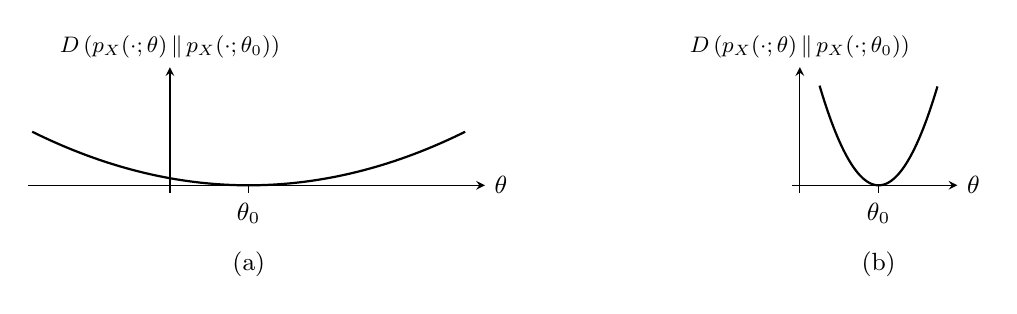
\begin{tikzpicture}
\shorthandoff{>}
%
\pgfmathsetmacro{\t}{1}
\pgfmathsetmacro{\dx}{8}
%
% peque�a curvatura
\draw[>=stealth,->] (-1.8,0)--(4,0) node[right]{\small $\theta$};
\draw[>=stealth,->] (0,-.1)--(0,1.5) node[above,scale=.9]
{\small $D\left( p_X(\cdot;\theta) \, \| \, p_X(\cdot;\theta_0) \right)$};
\draw[thick,domain=-1.75:3.75,samples=200] plot (\x,{.09*abs(\x-\t)^2});
\draw (\t,0)--(\t,-.1) node[below]{\small $\theta_0$};
%
% granda curvatura
\draw[>=stealth,->] ({-.1+\dx},0)--({2+\dx},0) node[right]{\small $\theta$};
\draw[>=stealth,->] (\dx,-.1)--(\dx,1.5) node[above,scale=.9]
{\small $D\left( p_X(\cdot;\theta) \, \| \, p_X(\cdot;\theta_0) \right)$};
\draw[thick,domain=.25:1.75,samples=200] plot ({\x+\dx},{2.25*abs(\x-\t)^2});
\draw ({\t+\dx},0)--({\t+\dx},-.1) node[below]{\small $\theta_0$};
%
\draw (\t,-1) node{\small (a)};
\draw ({\t+\dx},-1) node{\small (b)};
\end{tikzpicture} \end{center}
%
\leyenda{Ilustraci\'on         del        comportamiento         local        de
  $\Dkl[p_X(\cdot;\theta)]{p_X(\cdot;\theta_0)}$ \ en  funci\'on de \ $\theta$ \
  en \ $\theta_0$ \ en el contexto escalar \ $\Theta \subseteq \Rset$.  (a) Caso
  con \ $J_{\theta_0}(X)$  ``peque\~no'' \ y (b) caso  con \ $J_{\theta_0}(X)$ \
  ``grande''.   En  el caso  (b),  la determinaci\'on  de  \  $\theta$ \  usando
  $\Dkl{}$ \ va a  ser m\'as ``sencillo'' que en el caso  (a) porque el m\'inimo
  es m\'as ``picado''.}
%
\label{Fig:SZ:JCurvatura}
\end{figure}


% ----- de Bruijn

\subsubseccion{Identidad de de Bruijn}
\label{Sssec:SZ:DeBruijn}


Un otro  v\'inculo entre el  mundo de la  informaci\'on y el de  la estimaci\'on
aparece a trav\'es de la identidad  de de Bruijn~\footnote{A pesar de que tom\'o
  este nombre, esta identidad en su primera versi\'on fue publicada por Stam. En
  su papel~\cite{Sta59}, menciona que  esta identidad fue comunicada al Profesor
  van  Soest por el  Profesor de  Bruijn.}~\cite{Sta59, CovTho06,  Joh04, Bar84,
  Bar86,  PalVer06, TorZoz18}.  Esta  identidad caracteriza  lo que  es conocido
como  canal gaussiano  de la  figura Fig~\ref{Fig:SZ:deBruijnVerdu}-(a),  \ie la
salida \ $Y$ \ es una versi\'on ruidosa de la entrada.  La identidad vincula las
variaciones  de  entrop\'ia de  salida  con  respeto al  nivel  de  ruido, y  la
informaci\'on de Fisher.

\begin{figure}[h!]
%
\begin{center} 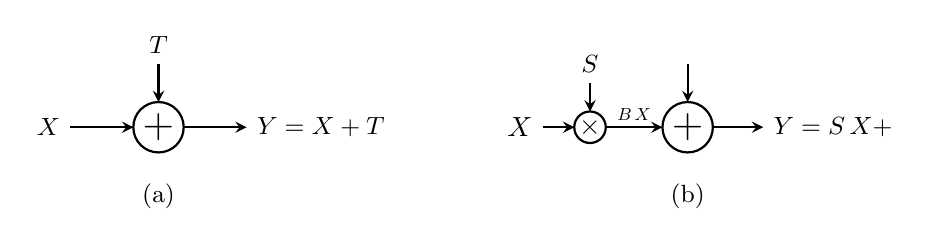
\begin{tikzpicture}[scale=.8]
\shorthandoff{>}
%
\begin{scope}
\draw[>=stealth,->,thick] (0,0) node[left]{\small $X$} --(1,0);
\draw[thick] (1.4,0) circle (.4);
\draw[>=stealth,->,thick] (1.4,1) node[above]{\small $T \N$} --(1.4,.4);
\node[align=center,scale=1.25] at (1.4,0){\large +};
\draw[>=stealth,->,thick] (1.8,0)--(2.8,0) node[right]{\small $Y = X + T \N$};
%
\end{scope}
%
\begin{scope}[xshift=7.5cm]
\draw[>=stealth,->,thick] (0,0) node[left]{$X$} --(.5,0);
\draw[thick] (.75,0) circle (.25);
\node[thick,align=center] at (.75,0){$\times$};
\draw[>=stealth,->,thick] (.75,.7) node[above]{\small $S$} --(.75,.25);
\draw[>=stealth,->,thick] (1,0)--(1.9,0);
\node[thick,align=center,scale=.7,above] at (1.45,0){\small $B \, X$};
\draw[thick] (2.3,0) circle (.4);
\draw[>=stealth,->,thick] (2.3,1) node[above]{\small $\N$} --(2.3,.4);
\node[align=center,scale=1.25] at (2.3,0){\large +};
\draw[>=stealth,->,thick] (2.7,0)--(3.5,0) node[right]{\small $Y = S \, X + \N$};
%
\end{scope}
\node at (1.4,-1.1){\small (a)};
\node at (9.8,-1.1){\small (b)};
\end{tikzpicture}
 \end{center}
%
\leyenda{Canal  de  comunicaci\'on  gaussiano  de  entrada  \  $X$.   (a)  Canal
  gaussiano usual, donde \ $T$ \ maneja los par\'ametros (nivel) del ruido.  (b)
  canal gaussiano con un preprocesamiento \ $S$ \ de la entrada.}
%
\label{Fig:SZ:deBruijnVerdu}
\end{figure}

\begin{teorema}[Identidad de de Bruijn]
\label{Teo:SZ:DeBruijn}
%
  Sea \ $X$ \  un vector aleatorio continuo sobre un abierto  de \ $\Rset^d$ \ y
  admitiendo una matriz de covarianza, y sea \  $Y = X + T \Gauss$ \ donde \ $T$
  \ es determinista, $d  \times d'$ \ con \ $ d \le d'$,  de rango m\'aximo, y \
  $\Gauss$ \  un vector  gaussiano centrado y  de covarianza  \ $\Sigma_\Gauss$,
  independiente  de \  $X$ \  (ver  figura Fig.~\ref{Fig:SZ:deBruijnVerdu}-(a)).
  Entonces, la  entrop\'ia de Shannon  y la informaci\'on  de Fisher de \  $Y$ \
  satisfacen
  %
  \[
  \nabla_T H(Y) = J(Y) \, T \, \Sigma_\Gauss,
  \]
  %
  donde \ $\nabla_T \, \cdot$ \ es la matriz de componentes \ $\frac{\partial \,
    \cdot}{\partial T_{i,j}}$.  Si \ $T = T(\theta)$ \ depende de un par\'ametro
  escalar~\footnote{Si el  par\'ametro es  multivariado, hace falta  entender la
    desigualdad a trav\'es de derivas parciales con respeto a los componentes de
    $\theta$.}  $\theta$,
  %
  \[
  \frac{\partial}{\partial \theta}  H(Y) = \Tr\left( J(Y) \,  T \, \Sigma_\Gauss
    \, \frac{\partial T^t}{\partial \theta} \right).
  \]
\end{teorema}
%
\begin{proof}
  La clave de este resultado viene del hecho  de que la densidad \ $p$ \ de \ $T
  \Gauss$ \ satisface una  ecuaci\'on diferencial particular.  La distribuci\'on
  de  \ $T  \Gauss$  \ se  escribe \  $p(x)  = (2  \pi)^{-\frac{d}{2}} \left|  T
    \Sigma_\Gauss  T^t  \right|^{-\frac12} \exp\left(  -  \frac12  x^t \left(  T
      \Sigma_\Gauss T^t \right)^{-1} x \right)$ \  (el rango m\'aximo de \ $T$ \
  asegura  que \  $T  \Sigma_\Gauss T^t$  \  sea invertible).   Para una  matriz
  invertible $R$,  desarollando \ $|R|$  \ con respecto  a su l\'inea \  $i$, se
  obtiene que  \ $\frac{\partial |R|}{\partial R_{i,j}} =  R_{i,j}^*$ \ cofactor
  de  \ $R_{i,j}$,  dando por  la regla  de Cram\'er  \ $\nabla_R  |R| =  |R| \,
  R^{-t}$ \  (ver tambi\'en~\cite[cap.~1~\&~9]{MagNeu99}), es  decir \ $\nabla_R
  |R|^{-\frac12}   =  -\frac12   |R|^{-\frac12}  R^{-t}$.    De  $\frac{\partial
    |R|^{-\frac12}}{\partial     T_{i,j}}     =    \sum_{k,l}     \frac{\partial
    |R|^{-\frac12}}{\partial R_{k,l}}  \frac{\partial R_{k,l}}{\partial T_{i,j}}
  =   -\frac12    |R|^{-\frac12}   \sum_{k,l}   \left(    R^{-1}   \right)_{l,k}
  \frac{\partial R_{k,l}}{\partial T_{i,j}}$ \ con \ $R = T \Sigma_\Gauss T^t$ \
  (sim\'etrica) y c\'alculos b\'asicos se obtiene finalmente
  %
  \[
  \nabla_T  \left|   T  \Sigma_\Gauss  T^t  \right|^{-\frac12}  =   -  \left|  T
    \Sigma_\Gauss T^t \right|^{-\frac12} \left( T \Sigma_\Gauss T^t \right)^{-1}
  T \Sigma_\Gauss.
  \]
  %
  Adem\'as, de \ $\left( T  \Sigma_\Gauss T^t \right) \left( T \Sigma_\Gauss T^t
  \right)^{-1}  =  I$ \  viene  \  $\frac{\partial  \left( T  \Sigma_\Gauss  T^t
    \right)^{-1}}{\partial T_{i,j}} = -  \left( T \Sigma_\Gauss T^t \right)^{-1}
  \frac{\partial \left( T \Sigma_\Gauss  T^t \right)}{\partial T_{i,j}} \left( T
    \Sigma_\Gauss T^t \right)^{-1}$.  Usando le vector \ $\un_i$ \ con 1 en su \
  $i$-\'esima componente, y cero si no, se obtiene
  %
  \begin{eqnarray*}
  \frac{\partial \left( x^t \left( T \Sigma_\Gauss T^t \right)^{-1} x
  \right)}{\partial T_{i,j}} & = & - x^t \left( T \Sigma_\Gauss T^t \right)^{-1}
  \left( \un_i \un_j^t \Sigma_\Gauss T^t + T \Sigma_\Gauss \un_j \un_i^t \right) \left( T
  \Sigma_\Gauss T^t \right)^{-1} x\\[2.5mm]
  %
  & = & - 2 \, \un_i^t \left( T \Sigma_\Gauss T^t \right)^{-1} x x^t \left( T
  \Sigma_\Gauss T^t \right)^{-1} T \Sigma_\Gauss \un_j
  \end{eqnarray*}
  %
  usando la relaci\'on  \ $x^t A \un_k \un_l^t B  x = \un_l^t B x  x^t A \un_k =
  \un_k^t A^t x x^t  B^t \un_l$ \ (escalares comutan y un  escalar es igual a su
  transpuesta) y usando la simetr\'ia de \ $T \Sigma_\Gauss T^t$.  Eso significa
  que
  %
  \[
  \nabla_T \left( x^t \left( T \Sigma_\Gauss T^t \right)^{-1} x \right) = - 2 \,
  \left(  T \Sigma_\Gauss  T^t \right)^{-1}  x  x^t \left(  T \Sigma_\Gauss  T^t
  \right)^{-1} T \Sigma_\Gauss,
  \]
  %
  dando
  %
  \[
  \nabla_T p(x)  = \left( - \left(  T \Sigma_\Gauss T^t \right)^{-1}  + \left( T
      \Sigma_\Gauss  T^t   \right)^{-1}  x   x^t  \left(  T   \Sigma_\Gauss  T^t
    \right)^{-1} \right) T \Sigma_\Gauss \, p(x).
  \]
  %
  Tomando la Hessiana de \ $p$ \  con respeto a \ $x$ \ se obtiene sencillamente
  que \ $p$ \ satisface la ecuaci\'on diferencial
  %
  \[
  \nabla_T \, p = \Hess_x \, p \: T \, \Sigma_\Gauss.
  \]
  %
  Suponiende que  se puede intervertir derivadas  y integrales (ver~\cite{Bar84,
    Bar86}     donde     se      dan     condiciones     rigurosas,     y     el
  teorema~\ref{Teo:MP:IntegralParametro},
  pagina~\pageref{Teo:MP:IntegralParametro}),     $\displaystyle     p_Y(y)     =
  \int_{\Rset^d}  p_X(x)  \,  p(y-x)  \, dx$  \  (ver  ejemplo~\ref{Ej:MP:Suma},
  pagina~\pageref{Ej:MP:Suma})    \   satisface   tambi\'en    esta   ecuaci\'on
  diferencial, y adem\'as
  %
  \begin{eqnarray*}
  \nabla_T H(Y) & = & - \int_{\Rset^d} \nabla_T \, p_Y(y) \log p_Y(y)
  \, dy - \int_{\Rset^d} \nabla_T \, p_Y(y) \, dy\\[2.5mm]
  %
  & = & - \left( \int_{\Rset^d} \Hess_y \, p_Y(y) \log p_Y(y) \, dy \right) T \,
  \Sigma_\Gauss - \nabla_T \int_{\Rset^d} p_Y(y) \, dy\\[2.5mm]
  %
  & = & - \left( \int_{\Rset^d} \left( \Hess_y \Big( p_Y(y) \log p_Y(y) \Big) -
  \Hess_y \, p_Y(y) - \frac{\nabla_y \, p_Y(y) \, \nabla_y \, p_Y(y)^t}{p_Y(y)}
  \right) \, dy \right) T \, \Sigma_\Gauss\\[2.5mm]
  %
  & = & - \left( \int_{\Rset^d} \Hess_y \Big( p_Y(y) \log p_Y(y) \Big) \, dy -
  \int_{\Rset^d} \Hess_y p_Y(y) \, dy \right) T \, \Sigma_\Gauss \: + \: J(Y) \, T
  \, \Sigma_\Gauss
  \end{eqnarray*}
  %
  usando la  ecuaci\'on diferencial  en la  segunda l\'inea, el  hecho de  que \
  $p_Y$ \ suma a  1 en la tercera l\'inea (su gradiente  es cero entonces), y la
  definici\'on de la matriz de Fisher  en la \'ultima l\'inea. Usando el teorema
  de la  divergencia (intergraci\'on por partes) aplicada  respectivamente a los
  componentes de \ $\nabla_y p_Y \log  p_Y$ \ y \ $\nabla_y p_Y$, suponiendo que
  estos gradientes se cancelan en el borde del dominio de integraci\'on, los dos
  t\'erminos integrales  valen cero, lo que  cierra la prueba  de la desigualdad
  general.  Adem\'as,  si \ $T =  T(\theta)$, la segunda desigualdad  sigue de \
  $\frac{\partial   \cdot}{\partial    \theta}   =   \sum_{i,j}   \frac{\partial
    \cdot}{\partial   T_{i,j}}   \frac{\partial   T_{i,j}}{\partial  \theta}   =
  \Tr\left( \nabla_T \cdot \, \frac{\partial T^t}{\partial \theta} \right)$.
\end{proof}

La versi\'on  inicial de la identidad de  de Bruijn, con \  $\Sigma_\Gauss = I$,
que se escribe
%
\[
\frac{d}{d\theta}     H(X+\sqrt{\theta}    \Gauss)    =     \frac12    \Tr\left(
  J(X+\sqrt{\theta} \Gauss) \right),
\]
%
se recupera  en el caso particular  \ $T =  \sqrt{\theta} I$.  En este  caso, la
ecuac\'ion diferencial satisfecha por la densidad  de probabilidad \ $p$ \ es la
{\it  ecuaci\'on del  calor}.  Esta  desigualdad cuantifica  las  variaciones de
entrop\'ias   bajo  variaciones   de  ``niveles''   del  ruido   del   canal  de
comunicaci\'on. De una  forma, caracteriza la robustez del  canal con respeto al
nivel de ruido gaussiano (la gaussiana juega de nuevo un rol central ac\'a).

\

Existe una  otra forma  muy similar  de esta desigualdad  debido a  Guo, Shamai,
Verd\'u,  Palomar~\cite{GuoSha05, PalVer06,  TorZoz18}.  Esta  versi\'on vincula
a\'un m\'as el mundo  de la informaci\'on y el de la  estimaci\'on.  Del lado de
la  comunicaci\'on, consiste  a  caracterizar la  informaci\'on  mutua entre  la
entrada \ $X$ \ de un canal ruidoso y su  salida, \ $Y = S X + \Gauss$ \ donde \
$S$ \ coresponde a un pre-tratamiento antes de la salida. Eso es ilustrado en la
figura  Fig.~\ref{Fig:SZ:deBruijnVerdu}-(b).  Del lado  de la  estimaci\'on, uno
puede querer  estimar \ $X$  \ observando solamente  \ $Y$.  Es conocido  que el
estimador  que minimiza  el error  cuadr\'atico promedio  \  $\Esp\left[ \left|
    \widehat{X}(Y)  - X  \right|^2 \right]$  \  es la  esperanza condicional  \
$\widehat{X}(Y)   =    \Esp[X|Y]$~\cite{Kay93,   Rob07,   LehCas98}.     \   Una
caracter\'istica de un  estimador siendo su matriz de  covarianza, se notar\'a \
$\E(X|Y)  =  \Esp\left[  \left( X  -  \Esp[X|Y]  \right)  \left( X  -  \Esp[X|Y]
  \right)^t  \right]$ \  esta  matriz.  Sorpredentemente,  existe tambi\'en  una
identidad entre \ $I(X;Y)$ \ y \ $\E(X|Y)$:
%
\begin{teorema}[Identidad de Guo--Shamai--Verd\'u]
\label{Teo:SZ:GuoShamaiVerdu}
%
  Sea \ $X$ \ un vector aleatorio  continuo sobre un abierto de \ $\Rset^{d'}$ \
  y admitiendo una  matriz de covarianza, y sea \  $Y = S X +  \Gauss$ \ donde \
  $S$  es determinista,  $d  \times d'$,  y  \ $\Gauss$  \  un vector  gaussiano
  centrado  y de covarianza  $\Sigma_\Gauss$, independiente  de $X$  (ver figura
  Fig.~\ref{Fig:SZ:deBruijnVerdu}-(b)). Entonces, la informaci\'on mutua entre \
  $X$ \ e \ $Y$ \ y  la matriz de covarianza del estimador de error cuadr\'atico
  m\'inimo satisfacen
  %
  \[
  \nabla_S \, I(X;Y) = \Sigma_\Gauss^{-1} S \, \E(X|Y).
  \]
  %
  Si \ $S = S(\snr)$ \ depende de un par\'ametro escalar $\snr$,
  %
  \[
  \frac{\partial}{\partial \snr} I(X;Y) = \Tr\left( \Sigma_\Gauss^{-1} \, S \,
    \E(X|Y) \, \frac{\partial S^t}{\partial \snr} \right).
  \]
\end{teorema}
%
\begin{proof}
  Notando  que \ $p_{Y|X=x}  (y) =  (2 \pi)^{-\frac{d}{2}}  \left| \Sigma_\Gauss
  \right|^{-\frac12}  \exp\left( -\frac12  (y-S  x)^t \Sigma_\Gauss^{-1}  (y-Sx)
  \right)$   \   viene  \   $\nabla_S   \,   p_{Y|X=x}(y)   =  p_{Y|X=x}(y)   \,
  \Sigma_\Gauss^{-1}  (y -  S x)  x^t$ \  (ver  unos pasos  de la  prueba de  la
  identidad de de  Bruijn) as\'i que \ $\nabla_y  \, p_{Y|X=x}(y) = p_{Y|X=x}(y)
  \, \Sigma_\Gauss^{-1} (y - S x)$, dando
  %
  \[
  \nabla_S \, p_{Y|X=x}(y) = \nabla_y \, p_{Y|X=x}(y) x^t \qquad \mbox{y} \qquad
  \nabla_S \, p_{X,Y}(x,y) = \nabla_y \, p_{X,Y}(x,y) x^t
  \]
  %
  (multiplicando ambos lados por $p_X$). Ahora, \ $I(X;Y) = H(Y) - H(Y|X) = H(Y)
  - H(\Gauss)$ \ (de la independencia, cuando \ $X  = x$, \ $Y = S x + \Gauss$ \
  gaussiana de  misma convarianza que \  $\Gauss$ \ y  de promedio \ $S  x$ (ver
  ejemplo~\ref{Ej:MP:SumaCond}, pagina~\pageref{Ej:MP:SumaCond}), as\'i que
  %
  \begin{eqnarray*}
  \nabla_S I(X;Y) & = & \nabla_S H(Y)\\[2.5mm]
  %
  & = & - \int_{\Rset^d \times \Rset^{d'}} \nabla_S \Big( p_{X,Y}(x,y) \, \log
  p_Y(y) \Big) \, dx \, dy\\[2.5mm]
  %
  & = & - \int_{\Rset^d \times \Rset^{d'}} \nabla_S \, p_{X,Y}(x,y) \, \log p_Y(y) \,
  dx \, dy - \int_{\Rset^d \times \Rset^{d'}} p_{X|Y=y}(x) \, \nabla_S \, p_Y(y) \, dx \,
  dy\\[2.5mm]
  %
  & = & \int_{\Rset^d \times \Rset^{d'}} \nabla_y \, p_{X,Y}(x,y) \, x^t \log p_Y(y)
  \, dx \, dy - \int_{\Rset^d} \nabla_S \, p_Y(y) \, dy\\[2.5mm]
  %
  & = & - \int_{\Rset^d \times \Rset^{d'}} \nabla_y \, p_Y(y) x^t p_{X|Y=y}(x) \, dx
  \, dy\\[2.5mm]
  %
  & = & - \int_{\Rset^d} \nabla_y \, p_Y(y) \, \Esp\left[X^t | Y = y \right] \, dy
  \end{eqnarray*}
  %
  La  segunda l\'inea  viene  de la  escritura  de \  $H(Y)$  usando $p_Y$  como
  marginale de $p_{X,Y}$ en $x$ y intercambiando gradiente e integral (ver pasos
  de   la   prueba  de   la   desigualdad  de   de   Bruijn);   la  tercera   de
  $\frac{p_{X,Y}(x,y)}{p_Y(y)}  =   p_{X|Y=y}(x)$;  en  la  cuarta   se  usa  la
  ecuaci\'on  diferencial satisfecha  por  $p_{X,Y}$ en  la  primera integral  y
  integrando en $x$ en la segunda  integral; la quinta l\'inea se obtiene usando
  el teorema de  la divergencia (intergraci\'on por partes)  en la integraci\'on
  en $y$  de la primera  integral, e intercambiando  gradiente e integral  el la
  segunda ($p_Y$ sumando a 1, el t\'ermino se cancela). Adem\'as,
  %
  \begin{eqnarray*}
  \nabla_y p_Y(y) & = & \int_{\Rset^{d'}} \nabla_y \, p_{Y|X=x}(y) \, p_X(x) \,
  dx\\[2.5mm]
  %
  & = & - \Sigma_\Gauss^{-1} \int_{\Rset^{d'}} (y - S x) \, p_{Y|X=x}(y) \, p_X(x) \,
  dx\\[2.5mm]
  %
  & = & - \Sigma_\Gauss^{-1} \left( y - S \int_{\Rset^{d'}} x \, p_{X|Y=y}(x) \,dx
  \right) p_Y(y)\\[2.5mm]
  %
  & = & - \Sigma_\Gauss^{-1} \Big( y - S \Esp\left[X | Y=y \right] \Big) \, p_Y(y)
  \end{eqnarray*}
  %
  escribiendo $p_{Y|X=x}(y)  \, p_X(x) =  p_{X|Y=y}(x) \, p_Y(y)$ en  la tercera
  l\'inea. Esta ecuaci\'on permite escribir
  %
  \begin{eqnarray*}
  \nabla_S I(X;Y) & = & \Sigma_\Gauss^{-1} \int_{\Rset^d} \Big( y - S \Esp\left[X |
  Y=y \right] \Big) \Esp\left[X^t | Y=y \right] \, p_Y(y) \, dy\\[2.5mm]
  %
  & = & \Sigma_\Gauss^{-1} \left( \Esp\left[ Y \Esp\left[ X^t|Y \right] \right] - S
  \Esp\left[ \Esp\left[X | Y \right] \Esp\left[X | Y \right]^t \right]
  \right)\\[2.5mm]
  %
  & = & \Sigma_\Gauss^{-1} \left( \Esp\left[ Y X^t \right] - S \Esp\left[
  \Esp\left[X | Y \right] \Esp\left[X | Y \right]^t \right] \right)\\[2.5mm]
  %
  & = & \Sigma_\Gauss^{-1} S \left( \Esp\left[ X X^t \right] - \Esp\left[
  \Esp\left[X | Y \right] \Esp\left[X | Y \right]^t \right] \right)
  \end{eqnarray*}
  %
  la \'ultima l\'inea viniendo de $Y  = S X + \Gauss$ con $\Gauss$ independiente
  de  $X$ y  de  promedio 0.   La prueba  se  cierra notando  que \  $\Esp\left[
    \Esp[X|Y] \right]  = \Esp[X]$  \ y por  la formula de  K\"onig-Huyggens (ver
  cap\'itulo~\ref{cap:MP:TeoriaProbabilidades},
  subsecci\'on~\ref{Ssec:MP:Momentos}, pagina~\pageref{Ssec:MP:Momentos}).

  La  segunda identidad  viene de  \ $\frac{\partial  \cdot}{\partial  \snr} =
  \Tr\left(  \nabla_S \,  \frac{\partial S^t}{\partial  \snr} \right)$  \ (ver
  prueba de la identidad de de Bruijn).
\end{proof}
%
\noindent  La  primera versi\'on  de  esta  identidad se  recupera  con  \ $S  =
\sqrt{\snr}$, \ $\Sigma_\Gauss =  I$ \ y \ $X$ \ de  covarianza la identidad; $s$ \
es conocido como relaci\'on se\~nale/ruido en este caso.

Existen versiones a\'un m\'as completas  (con gradientes con respeto a la matriz
\  $\Sigma_\Gauss$  \  por  ejemplo)  que se  pueden  consultar  en~\cite{Joh04,
  PalVer06, PayPal09}.



% ----- Stam

\subsubseccion{Desigualdad de Stam}
\label{Sssec:SZ:Stam}


De la  desigualdad de  la potencia entr\'opica  y de  la identidad de  de Bruijn
surge  una otra  desigualdad implicando  la potencia  entr\'opica \  $N$ \  y la
informaci\'on de Fisher \ $J$.  Esta desigualdad es conocida como desigualdad de
Stam~\footnote{Como para  la identidad  de de Bruijn,  Stam mencion\'o  que esta
  desigualdad fue  comunicada al  Profesor van Soest  por el Profesor  de Bruijn
  quien  da una  prueba variacional  de la  desigualdad.}~\cite{CovTho06, Rio07,
  Sta59},     o    a    veces     ``desigualdad    isoperimetrica     para    la
entrop\'ia''~\cite{WanMad04}.
%
\begin{teorema}[Desigualdad de Stam]
\label{Teo:SZ:Stam}
%
  Sea  \  $X$   \  una  variable  aleatoria  continua   sobre  \  $\X  \subseteq
  \Rset^d$. Entonces,
  %
  \[
  N(X) \Tr\left( J(X) \right) \, \ge \, d,
  \]
  %
  con igualdad si y solamente si \ $X$ \ es gaussiano de covarianza proporcional
  a la identidad.
\end{teorema}
%
\begin{proof}
  De la desigualdad de la potencia entr\'opica se obtiene \ $N(X + \sqrt{\theta}
  \Gauss)  \ge N(X)  + \theta  \left| \Sigma_\Gauss  \right|^{\frac1d}$. Tomando
  $\Sigma_\Gauss =  I$, se  obtiene \ $\forall  \, \theta  > 0,$ \  $\frac{N(X +
    \sqrt{\theta} \Gauss) - N(X)}{\theta}  \ge 1$.  Entonces, tomando el l\'imite
  \ $\theta \to 0$, aparece  que \ $\left. \frac{d}{d\theta} N(X + \sqrt{\theta}
    \Gauss)   \right|_{\theta  =   0}  \ge   1$.   La   prueba  se   cierra  con
  $\frac{d}{d\theta}  N(X   +  \sqrt{\theta}   \Gauss)  =  \frac{1}{2   \pi  \e}
  \frac{d}{d\theta}  \exp\left( \frac2d  H(X +  \sqrt{\theta} \Gauss)  \right) =
  \frac2d  N(X +  \sqrt{\theta}  \Gauss) \frac{d}{d\theta}  H(X +  \sqrt{\theta}
  \Gauss) = d N(X +  \sqrt{\theta} \Gauss) \Tr\left( J(X + \sqrt{\theta} \Gauss)
  \right)$ \ (por la identidad de  de Bruijn).  Adem\'as, la igualdad se obtiene
  cuando se  alcanza la cota  de la desigualdad  de la potencia  entr\'opica, es
  decir cuando \ $X$ \ es gaussiano de varianza proporcional a la del ruido, que
  es la identidad en este caso.
\end{proof}
%
Se  puede  ver  de  nuevo  el  rol  central  que  juega  la  gaussiana  en  esta
desigualdad. Adem\'as, de la desigualdad  de Stam se puede deducir tamb\'ien las
versiones escalares de  la desigualdad de Cram\'er-Rao. Viene  del hecho de que,
dada una matriz de covarianza, la entrop\'ia \ $H(X)$ \ es m\'axima cuando \ $X$
\ es gaussiano.  Entonces, para cualquier  \ $X$ \ de covarianza \ $\Sigma_X$, \
$N(X) \le \left| \Sigma_X \right|^{\frac1d}$,  dando de la desiguldad de Stam, \
$\left| \Sigma_X \right|^{\frac1d} \Tr\left( J(X)  \right) \ge d$ \ (y las otras
versiones  escalares de  la relaci\'on  determinente-traza).  Como  se  lo puede
esperar, se  obtiene la igualdad si y  solamente \ $X$ \  es gaussiano (potencia
entr\'opica alcanzando su  cota superior) y de matriz  la identidad (desiguladad
de Stam se saturando).

Varias   otras  pruebas   de  la   desigualdad  de   Stam  pueden   provenir  de
generalizaciones~\cite{Ber12:06_1, Ber13, LutYan05, LutLv12, ZozPue17}.
%, por ejemplo debido a Lutwak o Bercher~\cite{Lut, Ber}.
  \SZ{La
  secci\'on ZZZ lo va a rapidamente evocar. Ver caso discreto Kagan~\cite{Kag01}.}


% ----- Fisher inequalities

\subsubseccion{Fisher aditividad, procesamiento de datos y convoluci\'on }
\label{Sssec:SZ:FisherIneq}

Adem\'as del  gr\'an n\'umero de relaciones  entre la informaci\'on  de Fisher y
otras medidas  informacionales, la  informaci\'on de Fisher  satisface tambi\'en
desigualdades en si  mismo, muy parecidas a las satisfechas  por la entrop\'ia o
informaci\'on mutua.

Primero,  al  imagen  de  la   entrop\'ia  condicional,  se  puede  definir  una
informaci\'on         condicional         al         imagen        de         la
definici\'on Def.~\ref{Def:SZ:entropiacondicional},
%
\begin{definicion}[Matriz informaci\'on de Fisher par\'ametrica condicional]
\label{Def:SZ:MatrizFisherParametricaCondicional}
%
  Sean  $X$ \  e \  $Y$ \  dos variables  aleatoria parametrizada  por  el mismo
  par\'ametro  $m$-dimensional,  $\theta   \in  \Theta  \subseteq  \Rset^m$,  de
  distribuci\'on de probabilidad conjunta $p_{X,Y}(\cdot,\cdot;\theta)$ continua
  sobre   $\X   \times   \Y$   su  soporte,   $p_{X|Y=y}(\cdot;\theta)$   la
  distribuci\'on condicional  de $X$ connociendo  $Y=y$ y $p_Y$  la distribuci\'on
  marginal.  Suponga que  estas  distribuciones sean  diferenciable en  $\theta$
  sobre  $\Theta$.  La  matriz de  Fisher de  $X$ condicionalmente  a $Y$  es el
  promedio   estad\'istico   sobre   $p_Y$   de   la   matriz   de   Fisher   de
  $p_{X|Y}(\cdot;\theta)$, es decir
  %
  \[
  J_\theta(X|Y)  = \Esp\left[ \Big(  \nabla_\theta \log  p_{X|Y}(X;\theta) \Big)
    \Big( \nabla_\theta \log p_{X|Y}(X;\theta) \Big)^t \right].
  \]
  %
  donde  $p_{X|Y}(\cdot;\theta)   =  \frac{p_{X,Y}(\cdot,Y;\theta)}{p_Y(Y)}$  es
  ac\'a una variable aleatoria.
\end{definicion}

De  esta  definici\'on,   es  sencillo  probar  de  que   la  matriz  de  Fisher
param\'etrica    sigue    una   regla    de    cadena    al    imagen   de    la
propiedad~\ref{Prop:SZ:cadena},
%
\[
J_\theta(X,Y) = J_\theta(X|Y) + J_\theta(Y).
\]
%
Adem\'as, si $X$ e $Y$ son independientes, la informaci\'on de Fisher es aditiva
de la  misma manera  que $H$ satisface  las propiedades~\ref{Prop:SZ:aditividad}
y~\ref{Prop:SZ:independenciacondicional}, \ie
%
\[
J_\theta(X|Y)  = J_\theta(X)  \quad \Leftrightarrow  \quad J_\theta(X,Y)  =  J_\theta(X) +
J_\theta(Y)   \quad  \Leftrightarrow   \quad  X   \:  \&   \:  Y   \:  \mbox{son
  independientes.}
\]
%
En particular,  tratando de una  secuencia $X =  \{ X_i \}_{i=1}^n$  de vectores
aleatorias  independientes   parametrizados  por  $\theta$,   $J_\theta(X)  =  n
J_\theta(X_i)$, lo que significa que estimando $\theta$ a partir de la secuencia
se   baja  a   la  taza   $1/n$  la   cota  de   Cram\'er-Rao.    Se  referir\'a
a~\cite{Fis25:07, Sta59,  Kay93, KagSmi99,  Joh04, CovTho06, Rio07}  entre otros
para estas propiedades.

De la regla de cadena, viene  obviamente la desigualdad siguiente, parecida a la
propiedad de super-aditividad~\ref{Prop:SZ:superaditividad},
%
\[
J_\theta(X_1,\ldots,X_n) \, \ge \,  J_\theta(X_i) \quad \forall \, 1 \le i \le n,
\]
%
y  una   desigualdad  de  procesamiento   de  datos  via  la   informaci\'on  de
Fisher~\cite{Zam98, Rio07, CovTho06, Fri04, KagSmi99}:
%
\begin{teorema}[Desigualdad de procesamiento de datos tipo Fisher]
\label{Teo:SZ:DesigualdadProcesamientoDatosFisher}
%
  Sea  $\theta  \mapsto  X  \mapsto   Y$  un  proceso  de  Markov  con  $\theta$
  determinista y $p_{X,Y}$ parametrizado por $\theta$, es decir en este contexto
  que, $p_{Y|X=x}$ no es parametrizado por $\theta$. Entonces
  %
  \[
  J_\theta(X) \ge J_\theta(Y),
  \]
  %
  con igualdad si y solamente si $\theta \mapsto Y \mapsto X$ es tambi\'en
  de Markov. En  particular,
  %
  \[
  \forall \, g, \quad J_\theta(X) \ge J_\theta(g(X)).
  \]
  %
\end{teorema}
%
\begin{proof}
  De la regla de cadena tenemos
  %
  \[
  J_\theta(Y|X) + J_\theta(Y) = J_\theta(X|Y) + J_\theta(X).
  \]
  %
  Del hecho de que $p_{Y|X=x}$ no  es parametrizado por $\theta$ es sencillo ver
  que  $J_\theta(Y|X)  =  0$,  la  prueba  se  cerrando  de  $J_\theta(X|Y)  \ge
  0$. Adem\'as se obtiene la igualdad  si y solamente si $J_\theta(X|Y) = 0$, es
  decir de  la ``positividad'' del  integrante dando la  matrix de Fisher,  si y
  solamente si $p_{X|Y=y}$ no es parametrizado por $\theta$.
\end{proof}

Mencionamos de que existe tambi\'en una desigualdad parecida a la de la potencia
entr\'opica,  teorema~\ref{Teo:SZ:EPI}, dada en  el caso  escalar en~\cite{Joh04,
  Bla65, Zam98, DemCov91, KagYu08}:
%
\begin{teorema}[Desigualdad convolucional de Fisher]
\label{Teo:SZ:DesigualdadConvolucionalFisher}
%
  Sean  $X$  e  $Y$  dos variables  $d$-dimensionales  continuas  independientes
  parametrizadas.  Entonces
  %
  \[
  \forall \, a \in [0 \;  1], \quad J\left( \sqrt{a} \, X + \sqrt{1-a} \, Y
  \right) \, \le \, a \, J(X) + (1-a) \, J(Y),
  \]
  %
  con igualdad si y  solamente si \ $X$ \ e \ $Y$  \ son gaussianas con matrices
  de covarianza proporcionales, $\Sigma_Y \propto \Sigma_X$.
\end{teorema}
%
\begin{proof}
  $X$  \  e  \  $Y$  \  siendo  independientes,  tenemos  para  $W  =  X  +  Y$,
  $\displaystyle p_W(w)  = \int_\X p_X(x)  p_Y(w-x) \, dx$ convoluci\'on  de las
  distribuciones  de  \  $X$  \   y  de  \  $Y$  (ver  ejemplo~\ref{Ej:MP:Suma},
  pagina~\pageref{Ej:MP:Suma}).  Escribiendo $S_X =  \nabla_x \log p_X$ el score
  de $X$ y lo mismo para $Y$ y $W$,
  %
  \begin{eqnarray*}
  S_W(w) & = & \int_\X \frac{p_X(x)}{p_W(w)} \, \nabla_w p_Y(w-x) \, dx\\[2.5mm]
  %
  & = & - \int_\X \frac{p_X(x)}{p_W(w)} \, \nabla_x p_Y(w-x) \, dx\\[2.5mm]
  %
  & = & \int_\X \frac{p_Y(w-x)}{p_W(w)} \, \nabla_x p_X(x) \, dx\\[2.5mm]
  %
  & = & \int_\X \frac{p_Y(w-x) p_X(x)}{p_W(w)} \, \nabla_x \log p_X(x) \, dx\\[2.5mm]
  %
  & = & \int_\X p_{X|W=w}(w) \, \nabla_x \log p_X(x) \, dx\\[2.5mm]
  %
  & = & \Esp\left[ \left. S_X(X) \right| W = w \right]
  \end{eqnarray*}
  %
  Intercambiando  los roles de  \ $X$  \ e  \ $Y$,  tenemos tambi\'en  $S_W(w) =
  \Esp\left[ \left. S_Y(Y) \right| W =  w \right]$, as\'i que, para cualquier $0
  \le a \le 1$,
  %
  \[
  S_W(w) = \Esp\left[ \left. a S_X(X) + (1-a) S_Y(Y) \right| W = w \right].
  \]
  %
  A    continuaci\'on,    de     la    formula    de    K\"onig-Huyggens    (ver
  cap\'itulo~\ref{cap:MP:TeoriaProbabilidades},
  subsecci\'on~\ref{Ssec:MP:Momentos}, pagina~\pageref{Ssec:MP:Momentos}),
  %
  \[
  S_W(w) S_W(w)^t \: \le \:  \Esp\left[ \left. \left(a S_X(X) + (1-a) S_Y(Y)
      \right) \left(a S_X(X) + (1-a) S_Y(Y) \right)^t \right| W = w \right],
  \]
  %
  es decir, tomando el promedio en $W$,
  %
  \[
  J(X+Y) \: \le  \: a^2 J(X) + (1-a)^2 J(Y) +  a (1-a) \left( \Esp\left[
      S_X(X) S_Y(Y)^t \right] + \Esp\left[ S_Y(Y) S_X(X)^t \right] \right).
  \]
  %
  Luego, \ $X$ \ e \ $Y$ \  siendo independientes, $S_X(X)$ \ y \ $S_Y(Y)$ \ son
  tambi\'en independientes. Adem\'as son centradas, probando que el t\'ermino en
  $a  (1-a)$ vale  cero, dando  una  versi\'on equivalente  del teorema;  La
  versi\'on dada se recupera re-emplazando \ $X$ \ por \ $\sqrt{a} \, X$ \ e \
  $Y$ \ por \ $\sqrt{1-a} \, Y$.

  Escribiendo la desigualdad viniendo de la formula de K\"onig-Huyggens, se nota
  de que  la igualdad es  satisfecha si y  solamente si $a S_X(w-x)  + (1-a)
  S_Y(x) =  S_W(w)$ para cualquier  $x, w$. Integrando  en $x$ se  obtiene $-a
  \log  p_X(w-x) + (1-a)  \log p_Y(x)  = x  S_W(w) +  g(w)$. Derivando  en $w$
  obtenemos $-a \nabla_w \log p_X(w-x) = S_W(w) + \nabla_w g(w)$, es decir, en
  $w = 0$, notando de que $\nabla_w \log p_X(w-x) = -\nabla_x \log p_X(w-x)$, se
  nota de  que $\nabla_x  \log p_X(x)$ es  constante, \ie $X$  es necesariamente
  gausiana.  Similarmente, $Y$ es  necesariamente gausiana  tambi\'en. Adem\'as,
  calculando las informaciones de Fisher  en el caso gausiano, obtenemos $\left(
    \Sigma_X + \Sigma_Y \right)^{-1} =  \Sigma_X^{-1} + \Sigma_Y^{-1}$ lo que es
  posible si y solamente si $\Sigma_X$ \ y \ $\Sigma_Y$ \ son proporcionales.
\end{proof}
%
Este teorema tiene varias consecuencias.  En particular, interviene en la prueba
de la desigualdad de la potencia entr\'opica.

\

\SZ{  (2) ver MinFisher Frieden p. 235, Berchet Vignat 2009, Ernst 2017; cf. travaux
  rederivant MQ de Frieden-Plastino-Soffer  (1999, 2002), Reginato 98, Bickel 81
}